% Copyright (C) 2008, 2009, 2010, 2011, 2012, 2013, 2014 
% Bert Burgemeister
%
% Permission is granted to copy, distribute and/or modify this
% document under the terms of the GNU Free Documentation License,
% Version 1.2; with no Invariant Sections, no Front-Cover Texts and
% no Back-Cover Texts. For details see file COPYING.
%

\newcommand{\maintitle}{Cheatsheet By Hebi}
\newcommand{\AUTHOR}{Hebi Li}
%
%%%%%%%%%%%%%%%%%%
% pdf info
\newcommand{\SUBJECT}{Common\ Lisp}
\newcommand{\KEYWORDS}{{clqr cheatsheet lisp reference booklet}}
%
%%%%%%%%%%%%%%%%%%
% To be reset in paper-*.tex if there is plenty of room
\newcommand{\clearpagebeforeindex}{}
%
%
\documentclass[8pt,pagesize,twoside,footinclude=false,headinclude=false]{scrartcl}
%
%
%%%%%%%%%%%%%%%%%%

% outsourced page dimensions for letter paper
\setlength{\paperwidth}{4.25in}
\setlength{\paperheight}{11in}
%%\areaset[10mm]{8cm}{29cm}
\typearea[3mm]{20}
\renewcommand{\clearpagebeforeindex}{\clearpage}

% outsourced page dimensions for A4 paper
% \setlength{\paperwidth}{10.5cm}
% \setlength{\paperheight}{29.7cm}
% %%\areaset[10mm]{8cm}{29cm}
% \typearea[3mm]{20}
% \renewcommand{\clearpagebeforeindex}{\clearpage}



% outsourced hypertext colors
% for the printer-friendly version
\newcommand{\linkcolor}{black}
\newcommand{\urlcolor}{black}
\newcommand{\bookmarks}{false}
\newcommand{\pdfpagelayout}{SinglePage}
% outsourced hypertext colors
% for the screen-only version
% \newcommand{\linkcolor}{Fuchsia}
% \newcommand{\urlcolor}{MidnightBlue}
% \newcommand{\bookmarks}{true}
% \newcommand{\pdfpagelayout}{TwoColumnLeft}

%%%%%%%%%%%%%%%%%%
%

\usepackage{tikz}
\usetikzlibrary{shapes.multipart}
\usetikzlibrary{patterns}
\usetikzlibrary{positioning,fit,calc}
\usetikzlibrary{decorations.pathmorphing}
\usetikzlibrary{decorations.pathreplacing}
\usetikzlibrary{quotes}
\usetikzlibrary{graphs}
\usetikzlibrary{arrows.meta}



\usepackage{amsmath}
\usepackage{amsfonts}
\usepackage{amssymb}

\usepackage[mathcal]{euscript}


\usepackage{rotating}
\usepackage{graphicx}
\usepackage{multicol}
\usepackage{textcase}
% (HEBI: cannot load color again because perhaps the tikz package loaded it)
% \usepackage[usenames,dvips]{color}
\usepackage{suffix}
\usepackage{makeidx}
% (HEBI: and these colors needs color package, so move tikz above)
\definecolor{frontcovergray}{gray}{.85}
\definecolor{backcovergray}{gray}{.9}
\usepackage[pagestyles]{titlesec}
\usepackage{titletoc}


% my packages
\usepackage{listings}
\usepackage{textcomp}
\usepackage[inline]{enumitem}
\usepackage{courier}
\usepackage{indentfirst} % indent first paragraph after section
\usepackage{ulem}




%
%%%%%%%%%%%%%%%%%%
% Two font alternatives:
% (A) All (except cover pages) Computer Modern --
%     everything comes from the same sound root; gets about 5% longer
%     than alternative (B) 
\usepackage{type1cm}
\usepackage{exscale}
%%%%%%%%%%%%%%%%%%
% (B) Times mixed with Helvetica --
%     different sources; need scaling as they don't even agree in
%     their concept of height
%\usepackage{mathptmx}
%\usepackage[scaled]{helvet}
%%%%%%%%%%%%%%%%%%
%

% should remain last usepackage:
% \usepackage [breaklinks,linktocpage,colorlinks,
% bookmarksnumbered,bookmarks=\bookmarks,
% linkcolor=\linkcolor,urlcolor=\urlcolor,
% pdfpagelayout=\pdfpagelayout,
% pdftitle=\maintitle,pdfauthor=\AUTHOR,
% pdfsubject=\SUBJECT,pdfkeywords=\KEYWORDS]
% {hyperref}

%% it seems that I have to use this without those options to have the
%% outline. Not sure which one caused it.
\usepackage{hyperref}

\makeindex

%% I have to uncomment these two settings because they cause no outline
% \titleformat{\section}{\sffamily\mdseries\slshape}
%             {\huge\thesection}{.7em}{\huge}[{\titlerule[0.25pt]}]
            
% \titleformat{\subsection}{\sffamily\mdseries\slshape}
%             {\Large\thesubsection}{.7em}{\Large}[{\titlerule[0.25pt]}]

% Kill toc header as we want it to span columns
\deftocheading{toc}{}

\titlecontents{section}%
[1.5em]%
{\vspace{.5em plus 1em minus .2em}\sffamily\bfseries\upshape\filright}%
{\contentslabel{1.5em}}%
{\hspace*{3em}}%
{\hfill\contentspage\vspace{.1em}}%

\titlecontents{subsection}%
[4em]%
{\sffamily\mdseries\upshape\filright}%
{\contentslabel{2.5em}}%
{\hspace*{5.5em}}%
{\hspace{.5ex plus .5ex minus .3ex}\titlerule*[1em]{.}\contentspage}%





%% my settings
\lstset{upquote=true} % for back quote, need textcomp
\lstset{basicstyle=\ttfamily\small,breaklines=true}
% \lstset{frame=b}
% \lstset{float,floatplacement=H,captionpos=b}
% \lstset{numbers=left}
% \lstset{language=C}
\lstset{showstringspaces=false}
% \lstset{framextopmargin=10pt}
% \lstset{framextopmargin=50pt,frame=t}
% \lstset{float=htb,language=C,frame=single, basicstyle=\small, stringstyle=\ttfamily}
% \lstset{escapeinside={(*@}{@*)}}

\setlist[description]{nosep
  ,style=sameline,leftmargin=3cm
  ,font=\ttfamily
}
\setlist[itemize]{nosep}
\setlist[enumerate]{nosep}

\newlist{inlineitemize}{itemize*}{1}
\newlist{inlineenumerate}{enumerate*}{1}
\newlist{inlinedescription}{description*}{1}

% I have to have the setlist* to make it work
% and this only works for enumerate
\setlist*[inlineenumerate,1]{label=(\roman*)}

\newcommand{\NT}[1]{\textnormal{\texttt{#1}}}

              
% \input{clqr.macros}
%
\begin{document}

\newlength{\titlepagewidth}
\setlength{\titlepagewidth}{8cm}
%%%%%%%%%%%%%%%%%%%%%%%%%%%%%%%%%%%%%%%%%%%%%%%%%%
%% Front Cover
%%%%%%%%%%%%%%%%%%%%%%%%%%%%%%%%%%%%%%%%%%%%%%%%%%
\begin{titlepage}
  \renewcommand{\rmdefault}{ptm} %% Always times fonts on title
  \advance\oddsidemargin by 1.5mm
  \vspace*{15mm}
  \begin{center}
    \begin{minipage}{\titlepagewidth}
      \begin{center}
        \rmfamily\mdseries\itshape\fontsize{20}{0}\selectfont
        An Open Cheat Sheet to be precise and consistent\index{CLQR}\\
      \end{center}
    \end{minipage}
    \vfill
    \begin{minipage}{\titlepagewidth}
      \begin{center}
        \rmfamily\mdseries\itshape%
        \fontsize{200}{0}\selectfont{\color{frontcovergray}OS\/}\\
      \end{center}
    \end{minipage}
    \vfill
    \begin{minipage}{\titlepagewidth}
      \rmfamily\mdseries\itshape\fontsize{36}{0}\selectfont
      \hfill Open\/\\[2mm]
      \rmfamily\mdseries\upshape\fontsize{107}{0}\selectfont
      \rule[0mm]{\textwidth}{1.5mm}\\
      Sheat\\[1mm]
      \rule[15mm]{\textwidth}{1.5mm}\\
      % \rule[15mm]{5.5cm}{1.5mm}\hfill\rule[15mm]{1.77cm}{1.5mm}
    \end{minipage}\\
    \begin{minipage}{\titlepagewidth}
      \rmfamily\mdseries\upshape\fontsize{14}{0}\selectfont
      \AUTHOR
      \vspace*{4mm}
    \end{minipage}
  \end{center}

\end{titlepage}

%%%%%%%%%%%%%%%%%%%%%%%%%%%%%%%%%%%%%%%%%%%%%%%%%%
% TOC
%%%%%%%%%%%%%%%%%%%%%%%%%%%%%%%%%%%%%%%%%%%%%%%%%%
\section*{\contentsname}
\vspace{-3ex}
{%
  \setlength{\columnsep}{1.5em}%
  \begin{multicols}{2}
    \tableofcontents
  \end{multicols}%
}
%%%%%%%%%%%%%%%%%%%%%%%%%%%%%%%%%%%%%%%%%%%%%%%%%%
\vfill
%%%%%%%%%%%%%%%%%%%%%%%%%%%%%%%%%%%%%%%%%%%%%%%%%%
%%%%%%%%%%%%%%%%%%%%%%%%%%%%%%%%%%%%%%%%%%%%%%%%%%
%%%  CONTENT STARTS HERE  %%%%%%%%%%%%%%%%%%%%%%%%
%%%%%%%%%%%%%%%%%%%%%%%%%%%%%%%%%%%%%%%%%%%%%%%%%%

\clearpage

% I use many descriptions, reduce the sep spacing
% \global\setlength{\itemsep}{-5pt}

\section{Emacs}

\subsection{general}
\begin{description}
\item [list-face-displays]
\item [fill-region]
\item [list-package] open the \texttt{*package*} buffer, \texttt{Ux}
  to update all.
\item [helm-etags-select]
\end{description}

\subsection{help}
\begin{description}
\item [describe-key-briefly] \texttt{C-h c} command name for a key
  stroke.
\item [where-is] \texttt{C-h w}, shortcut for a command
\item [info] \texttt{C-h i} open the built-in info reader.
\item [view-echo-area-messages]
\end{description}

\subsection{Dired}
\begin{description}
\item [dired-next-subdir]
\item [dired-prev-subdir]
\item [dired-tree-up]
\item [dired-tree-down]
\end{description}

\subsection{window}
\begin{description}
\item [balance-window]
\item [toggle-window-split]
\end{description}

\subsection{file}
\begin{description}
\item [revert-buffer] Reload file on disk
\item [recover-file] recover from \texttt{\#xxx\#} file.
\item [read-only-mode] disable it to edit read only files
\end{description}

\subsection{edit}

\begin{description}
\item [replace-rectangle]
\item [upcase-word]
\item [downcase-word]
\item [transpose-words]
\item [transpose-lines]
\item [C-q xxx] insert a control sequence
\item [capitalize-word]
\item [fill-paragraph]
\item [fill-region]
\item [auto-fill-mode]
\item [zap-to-char]
\item [zap-up-to-char]
\item [ispell] check spell 
\item [flycheck] check on-the-fly
\end{description}

\subsection{programming}

\begin{description}
\item [checkdoc] check the warnings in doc string
\item [C-x C-e] evaluate
\item [C-u C-x C-e] evaluate and insert result
\item [C-M-a] move to the beginning of defun
\item [C-M-e] move to the end of defun
\item [C-M-h] mark defun
\item [C-M-f] move forward a sexp
\item [C-M-b] move backward a sexp
\item [C-M-k] kill a sexp
\item [C-M-t] transpose expressions
\item [C-M-<SPC>] mark following sexp
\item [C-M-n] move to the next sexp
\item [C-M-p] move to the previous sexp
\item [C-M-u] move up parenthesis
\item [C-M-d] move down parenthesis
\item [C-M-x] evaluate defun
\item [forward-sexp] forward semantic block
\item [backward-sexp]
\item [org-forward-heading-same-level] =C-c C-f=
\item [org-backword-heading-same-level] =C-c C-b=
\end{description}

\subsection{Marking}
\begin{description}
\item [exhange-point-and-mark]
\item [mark-word]
\item [mark-sexp]
\item [mark-paragraph]
\item [mark-defun]
\item [mark-page]
\item [mark-whole-buffer]
\item [set-mark-command] C-SPC, set mark, and activate it
\item [C-SPC C-SPC] set mark, but not activate it.
\item [C-u C-SPC] pop to previous mark in mark ring. current is stored
  at the end of mark ring(rotating)
\item [pop-global-mark] will store both position and buffer
\item [set the mark] \texttt{C-SPC C-SPC}, \texttt{C-w}, search
\end{description}

\subsection{Register}
\begin{description}
\item [point-to-register] save ppposition in a register
\item [jump-to-register]
\item [jump-to-register] the register can store a file
\item [copy-to-register]
\item [insert-register]
\end{description}


\subsection{Key Map}
To configure a specific key map.  Note that the =global-set-key= will
\textit{not} overwrite a specific key map, because the specific one has a
higher priority.

\begin{lstlisting}[language=lisp]
  (define-key org-mode-map (kbd "C-j")
    (lambda()
      (interactive)
      (join-line -1)))
\end{lstlisting}

\subsection{Variables}
\paragraph{File Local Variable}
Emacs looks for the following line on first line or second line if
first line is shebang. \texttt{mode} defines the major mode for this
file, while unlimited number of variables follows, separated by
\texttt{;}.

\begin{lstlisting}
-*- mode: Lisp; fill-column: 75; comment-column: 50; -*-=
\end{lstlisting}


A second way to specify file local variable is to have a ``local
variables list'' near the end of the file (no more than 3000
characters from the end of the file).  The =LocalXXX Variables:= and
=XXXEnd:= will be matched literally, so literal that I have to add XXX
to these $\ldots$
\begin{lstlisting}
This     /* Local XXX Variables:  */
Is       /* mode: c           */
Garbage  /* comment-column: 0 */
AuCTex   TeX-master: "cheatsheet"
Data     /* XXXEnd:           */
\end{lstlisting}

\paragraph{Directory Local Variable}
Put \texttt{.dir-locals.el} at the root directory, and it will be in
effect for all the files under that directory, recursively.  It should
be an associate list, the car can be either a mode name (or \texttt{nil}
applies to all modes) indicating the variables are for that mode, or a
sub-directory name to apply only in that directory.
\begin{lstlisting}[language=lisp]
((nil . ((indent-tabs-mode . t)
         (fill-column . 80)))
 (c-mode . ((c-file-style . "BSD")
            (subdirs . nil)))
 ("src/imported"
  . ((nil . ((change-log-default-name
              . "ChangeLog.local"))))))
\end{lstlisting}


\subsection{Info}
Info is a document system.  It is closely bundled with emacs, so I put
it here.  To install some new info document in the system, issue the
following commands (using =gnu-c-manual= as an example):

\begin{lstlisting}
# download the gnu-c-manual code
make gnu-c-manual.info
mv gnu-c-manual.info /usr/local/share/info
cd /usr/local/share/info
sudo install-info --info-file=gnu-c-manual.info --info-dir=.
\end{lstlisting}

\subsubsection{Info Operations}

\begin{description}
\item [SPC] page down, can cross node
\item [BACKSPACE] page up, can cross node
\item [M-n] \texttt{clone-buffer}, open a new info buffer
\item [n] next node on same level
\item [p] previous
\item [{[}] next node regardless of level
\item [{]}] previous
\item [u] up node
\item [l] back
\item [r] forward
\item [m] ~Info-menu~, convenient for search node title
\item [s] TODO search  a text in the whole info file
\item [i] TODO search indices only
\end{description}


\subsection{YASnippet}
Put this into latex-mode directory as a file named ``desc'', and run \texttt{yas-reload-all}.
\begin{lstlisting}[language=tex]
# -*- mode: snippet -*-
# name: desciption
# key: desc
# --
\begin{description}
$1
\end{description}
$2
\end{lstlisting}
% \subsection{Babel}
% How to write a \texttt{ob-xxx.el} file?

% \begin{enumerate}
% \item search org-mode babel, you will get a link:
%   http://orgmode.org/worg/org-contrib/babel/
% \item In this link, there's a "languages"
%   link. http://orgmode.org/worg/org-contrib/babel/languages.html
% \item Under "Develop support for new languages" section, there's link
%   to ob-template.el:
%   http://orgmode.org/w/worg.git/blob/HEAD:/org-contrib/babel/ob-template.el
% \item follow instruction to modify it.
% \end{enumerate}
% some good example to look at: ob-plantuml.el, ob-C.el

%%% Local Variables:
%%% TeX-master: "cheatsheet"
%%% End:

\clearpage
\section{Elisp}
\subsection{Concepts}

\subsubsection{Quote}
\begin{tabular}{@{}ll@{}}
  \lstinline!'! & read without evaluate \\
  \lstinline!`! & same as \lstinline!'! except it can partially evaluate.\\
  \lstinline!,! & evaluate inside back quote\\
  \lstinline!,@! & evaluate and splice the resulting list inside back quote.
\end{tabular}

\subsubsection{Symbol}
Three special forms define symbols: \texttt{defvar}, \texttt{defun}, and \texttt{defmacro}.
A symbol can not be both a function and macro, but it can be a variable and a function at the same time.

A symbol can have a property list.

\begin{tabular}{@{}ll@{}}
  \texttt{get <sym> <prop>} & get\\
  \texttt{put <sym> <prop> <val>} & set\\
  \texttt{symbol-plist <sym>} & return the p-list\\
  \texttt{setplist <sym> <plist>} & set p-list
\end{tabular}


\subsection{IO}
\begin{tabular}{@{}ll@{}}
  \texttt{print} & in quote, with newline before and after\\
  \texttt{prin1} & in quote\\
  \texttt{princ} & no addition\\
  \texttt{message} & display at bottom, goes into \lstinline!*Messages*! buffer
\end{tabular}


\subsection{Regular Expression}
\subsubsection{Syntax}
\paragraph{Basics}
\begin{tabular}{@{}ll@{}}
  \texttt{.} & everything except newline\\
  \texttt{*,+,?} & \\
  \texttt{*?,+?,??} & non-greedy, match the smallest part\\
  \texttt{} &\\
  \texttt{\lstinline![],[^],^,\$!} &
\end{tabular}


\paragraph{Character classes}
Use the double \texttt{[[]]} form. E.g. \texttt{[[:ascii:]]}, and also the negative writes \lstinline![^[:ascii:]]!.

\begin{tabular}{@{}ll@{}}
  \texttt{ascii} & 0-127\\
  \texttt{alnum} & letter or digit\\
  \texttt{alpha} & letter\\
  \texttt{blank} & space and tab\\
  \texttt{cntrl} & ASCII control char\\
  \texttt{digit} & 0-9\\
  \texttt{lower} & lower-case\\
  \texttt{upper} & upper-case\\
  \texttt{punct} & punctuation\\
  \texttt{space} & whitespace\\
  \texttt{word} & same as \lstinline!\w!
\end{tabular}

\paragraph{Backslash}
Backslash is also used in elisp read syntax. So when you want one \texttt{\\} in the string, you need to write double.

\begin{tabular}{@{}ll@{}}
  \lstinline!\w, \W, \b, \B! &\\
  \lstinline!\{\}! & \lstinline!{}! counter part\\
  \lstinline!\1! & either one of two expressions. Can be used in capturing group\\
  \lstinline!\(\)! & capturing group\\
  \lstinline!\(?:\)! & non-capturing group\\
  \lstinline!\(?NUM:\)! & numbered capturing group.. If conflict numbers, last one will win\\
  \lstinline!\DIGIT! & back reference
\end{tabular}

\paragraph{Syntax code}
\texttt{\\sCODE} can be used to refer to any character "whose syntax is CODE".
\texttt{\\SCODE} is the negative form.
See the "Syntax Class Table" chapter of elisp manual for details.

\begin{tabular}{@{}ll@{}}
  \lstinline!\s-! & whitespace\\
  \lstinline!\s[space]! & whitespace\\
  \lstinline!\sw! & \lstinline!\w!\\
  \lstinline!\s.! & punctuation\\
\end{tabular}

\subsubsection{Search}
\begin{description}
\item[regexp-quote \NT{str}] \uline{a regexp} whose only exact match is str.
\item[regexp-opt \NT{strs}] \uline{an \textit{efficient} regexp}
  matching any of the strings.
\item[re-search-forward \NT{reg}] 
\item[re-search-backward \NT{reg}] 
\item[string-match \NT{reg str}] \uline{index} of first match.
  Set \uwave{\textit{Match Data}}
\item[string-match-p \NT{reg str}] \uline{index} of first match.
\item[match-string \NT{idx}] \uline{component} of \textit{Match Data}, 0 for entire match
\item[match-beginning \NT{idx}] \uline{beginning index} of the \textit{Match Data}
\item[match-end \NT{idx}]
\item[replace-regexp-in-string \NT{regexp rep string}] \uline{a
    modified copy} with all matches replaced with \texttt{rep}.
\end{description}

\subsection{Type}
\subsubsection{Equal}
\begin{description}
\item [eq \textnormal{\texttt{o1 o2}}] \texttt{t} if same Lisp object. Faster than \texttt{equal}
\item [equal \textnormal{\texttt{o1 o2}}] \texttt{t} if similar structure and contents
\item [=] \texttt{t} if all args are \texttt{equal}. Only for numbers
\item [string=] compare two strings
\end{description}

\subsubsection{Number}
\begin{description}
\item [expt \NT{a b}] $a^b$
\end{description}

\subsubsection{String}
\begin{description}
%  construct
\item [make-string \NT{ct char}] make string by duplicating characters
\item [substring \NT{str start \&opt end}]
\item [concat \NT{\&rest sequences}]
\item [split-string \NT{str \&opt seps}] default seps: \verb!"[ \f\t\n\r\v]+"!
% convert
\item [number-to-string \NT{num}]
\item [string-to-number \NT{str}]
\item [char-to-string \NT{char}]
\item [string-to-char \NT{str}] returns the first character in string
% case
\item [downcase \NT{string-or-char}]
\item [upcase \NT{string-or-char}]
\item [capitalize \NT{string-to-char}]
\end{description}

\subsubsection{cons cell}
This is a pair of slots, each of them can hold anything.  A list is a
list of cons cells, in which each cdr is the "address" next list.
\textit{Destructive} operations mean the cdr of the cons cells are
modified.

A \textit{dotted pair notation} is a more general syntax of a cons
cell.  It is written as \texttt{(A . B)}.  It is more general because
the cdr can also hold anything.  As an example, \texttt{(1 2)} is
the same as \verb$(1 . (2 . nil))$.  If the CDR of a list’s
last cons cell is some value other than ‘nil’, we call the structure a
\textit{dotted list}, since its printed representation would use
dotted pair notation.

\begin{description}
% construct
\item [cons \NT{obj1 obj2}] create a \uline{cons cell} with args
  as CAR and CDR. If obj1 is a list, this is called \textit{cons obj2 onto the list}.
\item [list \NT{\&rest objs}] create a list
\item [make-list \NT{length obj}] make a list of \texttt{length}, each
  cell holding the \textit{same} object, using \texttt{eq}
\item [append \NT{\&rest seqs}] last one is a list. Concatenate into
  one list, all arguments except the last one are copied. Set
  \texttt{nil} to the last to force copy everything.
\item [reverse \NT{list}] reverse the list by copying
\item [number-sequence \NT{from to}] the list of \texttt{[from,to]}, inclusive

% access
\item [car,cdr]
\item [car-safe,cdr-safe]
\item [caar] car car, 11
\item [cadr,cdar,cddr]
\item [nth \NT{n list}] get the \uline{nth element}, starting from 0
\item [nthcdr \NT{n list}] execute \uline{cdr n times}
\item [last \NT{list}]
\item [pop] return the \uline{cdr}, and \uwave{remove it from the list}
\item [length]

% modify  
\item [push \NT{el list}] modify \uwave{\texttt{list}} by cons \texttt{el} onto it.
\item [add-to-list \NT{list el}] cons \texttt{el} onto \uwave{\texttt{list}}
  if it is not there.
\item [setcar \NT{cons obj}]
\item [setcdr \NT{cons obj}]
\item [sort \NT{list pred}] destructive due to rearrange the cdrs
\end{description}

\subsubsection{set}
We use list as set, by ignoring the order ...
\texttt{append} to combine two set, then \texttt{delete-dups} to remove duplication ...

\begin{description}
\item [memq \NT{obj list}] whether obj is a member of list, using \texttt{eq}
\item [delq \NT{obj list}] destructively remove all elements \texttt{eq} to obj.
\item [rmq obj \NT{list}] return a copy of list with all obj removed
\item [member] \texttt{equal} counter-part
\item [member-ignore-case] for string
\item [delete] \texttt{equal} counter-part
\item [remove] \texttt{equal} counter-part
\item [delete-dups] use \texttt{equal}
\end{description}

\subsubsection{association list}
This is a special list, each element is a key-value pair.

\begin{lstlisting}
(setq alist-of-colors
  '((rose . red) (lily . white) (buttercup . yellow)))
\end{lstlisting}


\begin{description}
\item [assoc \NT{key list}]
  \uline{first element} of \textit{list} whose car \texttt{equal} \textit{key}.
\item [rassoc \NT{val list}]
  \uline{first element} of \textit{list} whose cdr \texttt{equal} \textit{val}
\item [assq \NT{KEY list}]
  \uline{first element} of \textit{list} whose car \texttt{eq} \textit{key}.
\item [rassq]
  \uline{first element} of \textit{list} whose cdr \texttt{eq} \textit{val}
\item [assoc-string \NT{key list \&opt case-fold}] This is \texttt{assoc} for
  string. if \texttt{case-fold} is non-nil, case is ignore-d.

\item [copy-alist \NT{list}] two-level deep copy
\item [assq-delete-all \NT{key list}] delete all elements whose car \texttt{eq} \textit{key}
\item [rassq-delete-all \NT{val list}] delete all elements whose cdr \texttt{eq} \textit{key}
\end{description}

\subsubsection{property list}
It is a flat list. The odd elements are property name, and the even elements are values.

\begin{lstlisting}[language=lisp]
(pine cones numbers (1 2 3) color "blue")
\end{lstlisting}
The property names \textit{must} be unique.
The order of the "pairs" does not matter.
\begin{description}
\item [plist-get \NT{plst prop}] get the \uline{value}
\item [plist-put \NT{plst prop val}] set the \uwave{value of \texttt{plst}}
\item [lax-plist-get] use \texttt{equal}
\item [lax-plist-put] use \texttt{equal}
\item [plist-member \NT{plst prop}] return \uline{the tail of
    \texttt{plst} whose car is \texttt{prop} (non-nil)} if \texttt{prop} is in
  \texttt{plst}. This is useful because it can distinguish the missing
  property and the property with value \texttt{nil}
\end{description}


\subsubsection{sequence}

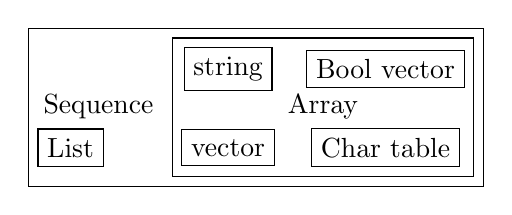
\begin{tikzpicture}
  % \node (A) [rectangle,draw,rounded corners] at (0,1) {hello};
  % \node (B) at (0,2) {yes};
  % \draw (0,1) -- (2,4);
  % \node [rectangle,draw,label=sequence] {
  %   % \node [label=list] {
  %   %   % \node [label="Array"] {};
  %   % };
  % };

  \node (vector) at (0,0) [draw] {vector};
  \node (string) at (0,1) [draw] {string};
  \node (char) at (2,0) [draw] {Char table};
  \node (bool) at (2,1) [draw] {Bool vector};
  \node (array) [draw,fit={(vector) (string) (char) (bool)},"center:Array"] {};
  \node (list) at (-2,0) [draw] {List};
  \node (sequence) [draw,fit={(list) (array)},label={[shift={(-2,0)}]center:Sequence}] {};
\end{tikzpicture}

\begin{description}
\item [length \NT{seq}]
\item [elt \NT{seq idx}] returns the element of \textit{seq} at \textit{index}
\item [copy-sequence \NT{seq}] the sequence is new, but the elements are not.
\end{description}

\subsubsection{array}
It is fixed length sequence.
\begin{description}
% constructing
\item [make-vector \NT{length object}] create vector
\item [vector \NT{\&rest objects}] create vector
% accessing
\item [aref \NT{array index}] getter
\item [aset \NT{array index object}] setter
\end{description}

\subsubsection{hash table}
\begin{description}
% construct
\item [make-hash-table]

% access
\item [gethash \NT{key table}]
\item [puthash \NT{key value table}]
\item [remhash \NT{key table}] remove
\item [clrhash \NT{table}] remove all
\item [maphash \NT{function table}] call function once for each of the
  element in table. The function should accept two arguments: key and
  value
% other
\item [hash-table-count \NT{table}] return number of entries
\end{description}

\subsection{Function}

\begin{description}
  % define
\item [defun \NT{name arglst \&opt docstr decl \&rest body}]
\item [defmacro \NT{name args body}] Macro does not evaluate its
  arguments. It put the arguments /as is/ and put them into the macro
  body to form an expression.  The expression is then evaluated for
  result.

  % Anonymous functions
\item [lambda \NT{args body}]
\item [function \NT{fun-obj}] returns the function without evaluating
  it. It is the "quote" for function
\item [\#'] this is the read syntax for the above \texttt{function}
  special form. You see, it is indeed the \textit{quote} for the
  function.

  % Calling
\item [funcall \NT{fun \&rest args}] compute which function to execute
  at runtime
\item [apply \NT{fun \&rest args}] compute the arguments at
  runtime. Same as =funcall=, but the /last/ of arguments is a list,
  and will be expanded into many arguments instead of a list.

  % Mapping family
\item [mapcar \NT{fun seq}] execute function on each element of
  sequence, and return the list of results.
\item [mapc \NT{fun seq}] same as =mapcar= except it returns the
  =sequence=, with the intention to collect side effect.
\item [mapconcat \NT{fun seq sep}] execute function on
  elements of sequence. The results must be strings, and will be
  concatenated and returned.
\end{description}



\subsection{Control Structure}

\begin{description}
% Sequential
\item [progn \NT{forms...}] return the result of final form
\item [prog1 \NT{form1 forms...}] return the result of form1
\item [prog2 \NT{form1 form2 forms...}] return the result of form2
% Conditional
\item [not]
\item [and]
\item [or]
\item [if \NT{condition then-form else-forms...}]
\item [when \NT{condition then-forms...}]
\item [unless \NT{condition forms...}]
\item [cond \NT{clause...}] the clause must be a list:
  \texttt{(condition body-forms...)}.  It is not exactly the "case"
  statement, because the condition is evaluted to true or false.  Any
  remaining forms are \textit{ignored}.
\item [pcase \NT{exp branch1 branch2 branch3...}] this is more like
  the "case" statement. The EXP is first evaluted and compare with the
  car of each branches.  The branch must be of the form
  \texttt{(UPATTERN BODY-FORMS...)}
\item [while \NT{condition forms...}]
\item [dolist \NT{(var list [result]) body...}] execute body for each
  element of list, with the bound of var to the current element and
  result for return.
\item [dotimes \NT{(var count [result]) body...}] execute body for
  each index of \texttt{[0,count)}, with var bound to the index, and
  result bound for return.
\end{description}

\subsubsection{CL Loop facility}
The package cl-lib.el ports many common lisp facilities into elisp,
most importantly, the loop facility.  So this section, at least for
now, focus on \texttt{cl-loop}.

\begin{description}
\item [cl-loop \NT{clauses...}] general loop form.
\item [for \NT{var} from \NT{from} to \NT{to} by \NT{step}]
  \textit{from} defaults to 0. \textit{step} must be positive and default to 1;
  inclusive \texttt{[from,to]};
  \texttt{from} can be \texttt{upfrom} and \texttt{downfrom}. I think it is wired to use this;
  \texttt{to} can be \texttt{upto} and \texttt{downto}. This makes more sense;
  \texttt{above} and \texttt{below} can be used, but /exclusive/. e.g. \texttt{for var below 10}
\item [for VAR in LIST by FUNCTION] =FUNCTION= is used to traverse the list, defaults to =cdr=
\item [for VAR on LIST by FUNCTION] =VAR= is bound to the cons cell of the list instead of the element.
\item [for VAR across ARRAY] iterates all elements of array
\item [for VAR ]PR1 then EXPR2= :: this is the most general form.  The
  =VAR= is bound to =EXPR1= initially, and will be set by evaluating
  =EXPR2= in successive iterations.  =EXPR2= can refer the old =VAR=

% iteration clauses
\item [repeat \NT{integer}] repeat the loop how many times
\item [while \NT{condition}] stops the loop when the condition becomes nil
\item [until \NT{condition}]
\item [always \NT{condition}] like while except it returns =nil=, and =finally= clauses are not executed.
\item [never \NT{condition}] counter part for =always=

% accumulation clauses
\item [collect \NT{form}] collect into a list and return the list in the end
\item [append \NT{form}] collect the lists into a list by appending, and return it in the end
\item [concat \NT{form}] for string only
\item [count \NT{form}] count how many times form evaluates to non-nil.
\item [sum \NT{form}] sum all the values
\item [maximize \NT{form}] get the max. If the form is never executed, result is /undefined/
\item [minimize \NT{form}]

% Other clauses
\item [with var = value] set the value one-time at the beginning of
  the loop.  Often used as return variable.  *The spaces around ~=~ is
  essential!*.
\item [if condition clause [else clause]]
\item [when condition clause] same as if
\item [unless condition clause] similar
\item [initially [do] forms...] execute before the loop begins, but
  after the =for= and =with= variable bindings. =do= is optional.
\item [finally [do] forms...] execute after the loop finishes
\item [finally return form] finally return it ...
\item [do forms...] execute as an implicit =progn= in the body
\item [return form] this is often used in =if= or =unless=, because
put it in top level will cause the loop always execute only once.
\end{description}



\subsection{Debugging}
\subsubsection{lisp debugger}
The simplest debugger is called =lisp debugger=.
You can turn on the =debug-or-error= flag,
but I found inserting the =(debug)= command useful.
Simply insert =(debug)= where you want program to suspend, and run it.
You will enter the debugger at that point.
In the debugger buffer, the following commands are available:
\begin{description}
\item [c] continue run program
\item [d] step
\item [e] evaluate an prompt expression
\item [R] like =e=, but also save the result in =*Debugger-record*=
\item [q] quit
\item [v] toggle display of local variables ???
\end{description}
\subsubsection{Edebug}
For this to work, first you need to instrument the code.
You can instrument the defun by =C-u C-M-x=.
Actually this is adding a prefix before =eval-defun=,
which instrument, and then evaluate the defun.

After instrumentation, running the defun will cause the program to stop at the first /stop point/ of the function.
The /stop points/ are
\begin{itemize}
\item before and after each subexpression that is a list
\item after each variable reference
\end{itemize}

\begin{description}
\item [b] set a breakpoint. You can also set the /source breakpoints/, by adding =(edebug)=.
\item [u] unset a breakpoint
\item [x CONDITION] set a conditional breakpoint
\item [B] move point to the next breakpoint
\item [w] move point back to the current stop point
\item [<SPC>] run to next stop point
\item [g] execute until next breakpoint
\item [q] exit
\item [S] stop and wait for Edebug commands
\item [n] evaluate a sexp and stop at stop point
\item [t] /trace/, pause one second at each stop point ...
\item [T] rapid trace. Update the display at each stop point but don't actually pause ...
\item [c] pause one second at each breakpoint
\item [C] rapid continue.
\item [G] run and ignore breakpoints (but you can stop it by =S=)

\item [h] proceed to the stop point near the point ...
\item [f] run one expression
\item [o] step out the containing expression
\item [i] step in
\item [e EXP] evaluate a prompt expression
\item [C-x C-e] evaluate an expression at point
\item [?] show help
\item [r] redisplay the most recent sexp result
\item [d] display the backtrace
\end{description}


%%% Local Variables:
%%% TeX-master: "cheatsheet"
%%% End:

\clearpage
\section{\LaTeX}

\subsection{Installation}
To see what is your tex home: \texttt{kpsewhich -var-value=TEXMFHOME}
It should be something like "~/texmf".  Putting class and style file
into correct path inside that folder will enable global usage of the
class.  check whether it works or not: \texttt{kpsewhich
  sig-alternate-05-2015.cls} Typically you don't need to update
database, but if you want, Command to update the =ls-R= database:
\texttt{texhash} or \texttt{mktexlsr}

\begin{tabular}{@{}ll|ll@{}}
  \verb$\alpha$ & $\alpha$ & \verb$\theta$ & $\theta$ \\
  \verb$\phi$ & $\phi$ & \verb$\varphi$ & $\varphi$ \\
  \verb$\xi$ & $\xi$ & \verb$\mu$& $\mu$\\
  \verb$\pi$ & $\pi$ & \verb$\rho$ & $\rho$\\
  \verb$\sigma$ & $\sigma$ & \verb$\epsilon$ & $\epsilon$\\
  \verb$\partial$ & $\partial$\\
  \hline
  \verb$\quad$ & $\alpha\quad\beta$ & \verb$\qquad$ & $\alpha\qquad\beta$\\
  \hline
  \verb$\cup$ & $\cup$ & \verb$\bigcup$ & $\bigcup$ \\
  \verb$\cap$ & $\cap$ & \verb$\vee$ & $\vee$ \\
  \verb$\wedge$ & $\wedge$ & \verb$\in$ & $\in$ \\
  \verb$\notin$ & $\notin$ & \verb$\neg$ & $\neg$ \\
  \verb$\subset$ & $\subset$ & \verb$\subseteq$ & $\subseteq$\\
  \verb$\supset$ & $\supset$ & \verb$\supseteq$ & $\supseteq$ \\
  \verb$\le$ & $\le$ & \verb$\ge$ & $\ge$\\
  \verb$\neq$ & $\neq$ & \verb$\forall$ & $\forall$\\
  \verb$\exists$ & $\exists$\\
  \hline
  \verb$\leftarrow$ & $\leftarrow$ & \verb$\rightarrow$ & $\rightarrow$\\
  \verb$\Rightarrow$ & $\Rightarrow$ & \verb$\Leftarrow$ & $\Leftarrow$\\
  \verb$\Leftrightarrow$ & $\Leftrightarrow$ & \verb$\longrightarrow$ & $\longrightarrow$\\
  \hline
  \verb$\hat{a}$ & $\hat{a}$ & \verb$\vec{x}$ & $\vec{x}$\\
  \hline
  \verb$\infty$ & $\infty$ & \verb$\propto$ & $\propto$\\
  \verb$\lfloor$ & $\lfloor$ & \verb$\rfloor$ & $\rfloor$\\
  \verb$\lceil$ & $\lceil$ & \verb$\rceil$ & $\rceil$\\
  \verb$\sum$ & $\sum$ & \verb$\int$ & $\int$\\
  \verb$\ldots$ & $ \ldots$ & \verb$\frac{a}{b}$ & $\frac{a}{b}$\\
  \verb$\sqrt{n}$ & $\sqrt{n}$ & \verb$\overline{abc}$ & $\overline{abc}$\\
  \verb$\prod$ & $\prod$ & &  \\
  \hline
  \verb$\checkmark$ & $\checkmark$ & \verb$\times$ & $\times$\\
  \hline
  \verb$\tiny$ & \tiny tiny & \verb$\scriptsize$ & \scriptsize scriptsize\\
  \verb$\footnotesize$ & \footnotesize footnotesize& \verb$\small$ & \small small\\
  \verb$\normalsize$ & \normalsize normalsize& \verb$\large$ & \large large\\
  \verb$\Large$ & \Large Large& \verb$\LARGE$ & \LARGE LARGE\\
  \verb$\huge$ & \huge huge& \verb$\Huge$ & \Huge Huge
\end{tabular}



\subsubsection{General Syntax}

\begin{tabular}{@{}l|l|l@{}}
  \begin{lstlisting}
    \begin{enumerate}
    \item xxx
    \end{enumerate}
  \end{lstlisting} &
\begin{lstlisting}
  \begin{itemize}
  \item like this,
  \end{itemize}
\end{lstlisting}&
\begin{lstlisting}
  \begin{description}
  \item[Word] Definition
  \end{description}
\end{lstlisting}\\
\end{tabular}

\begin{tabular}{@{}l|l@{}}
\begin{lstlisting}
  \begin{table}
    \centering
    \begin{tabular}{l|r}
      Item & Quantity \\\hline
      Widgets & 42 \\
      Gadgets & 13
    \end{tabular}
    \caption{\label{tab:widgets}
      An example table.}
  \end{table}
\end{lstlisting} &
\begin{lstlisting}
  \begin{figure}
    \centering
    \includegraphics[width=0.3\textwidth]{frog.jpg}
    \caption{\label{fig:frog}caption.}
  \end{figure}
\end{lstlisting}
\end{tabular}

\begin{tabular}{@{}l|l@{}}
  \begin{lstlisting}
    \label{xxx}
    \ref{xxx}
    \label{xx:yy}
    \ref{xx:yy}
  \end{lstlisting}&
\begin{lstlisting}
\todo{comment in the margin!}
\todo[inline, color=green!40]{inline comment.}
\end{lstlisting}
\end{tabular}

\subsection{Special characters}
\begin{description}
\item [\textbackslash textbackslash] \textbackslash
\item [\textbackslash textasciitilde] \textasciitilde
\end{description}




\subsection{Package: listings}
Predefined languages:
Ada, Algol, Ant, Assembler, Awk, bash, Basic, C, C++, CIL, csh,
Delphi, Eiffel, erlang, Fortran, Gnuplot, Haskell, HTML, Java, Lisp,
LLVM, Lua, make, Matlab, Mercury, ML, Octave, Pascal, Perl, PHP,
PostScript, Prolog, Python, R, Ruby, S, Scala, sh, SQL, tcl, TeX,
VBScript, Verilog, VHDL, XML, XSLT


To make the code listing more pretty, the font needs to be changed.
\verb$\usepackage{courier}$.

global setting:

\begin{lstlisting}
\lstset{basicstyle=\ttfamily,breaklines=true}
% \lstset{frame=b}
\lstset{float,floatplacement=H,captionpos=b}
% \lstset{numbers=left}
\lstset{language=C}
\lstset{showstringspaces=false}
% \lstset{framextopmargin=10pt}
% \lstset{framextopmargin=50pt,frame=t}
% \lstset{float=htb,language=C,frame=single, basicstyle=\small, stringstyle=\ttfamily}
\lstset{escapeinside={(*@}{@*)}}
\end{lstlisting}

\subsection{Package: ulem}

\begin{description}
\item [\textbackslash sout] strike through
\end{description}


\subsection{Package: multicol}
\begin{lstlisting}
\usepackage{multicol}
\begin{multicols}{3}
\end{multicols}
\end{lstlisting}

\subsection{Package: enumitem}
\begin{lstlisting}
\usepackage{enumitem}
\setlist[description]{nosep,style=sameline,leftmargin=3cm,font=\ttfamily}
\setlist[itemize]{nosep,leftmargin=*}
\setlist[enumerate]{nosep}
\end{lstlisting}


%%% Local Variables:
%%% TeX-master: "cheatsheet"
%%% End:

\clearpage
\section{TikZ}

Use of tikz packages.

\begin{lstlisting}
\usepackage{tikz}
\usetikzlibrary{shapes.multipart}
\end{lstlisting}

You can generate picture as pdf file.  To generate figure, add the
following lines, and execute: \texttt{pdflatex -shell-escape
  helium.tex}

\begin{lstlisting}
\usetikzlibrary{external}
\tikzexternalize
\tikzset{external/force remake}
\end{lstlisting}

There's also some library not supported. They need luatex.
\begin{lstlisting}
\usetikzlibrary{graphs,graphdrawing}
\usegdlibrary{layered}
\end{lstlisting}

To create a tikz picture, use
\begin{lstlisting}
  \begin{figure*}[ht]
    \centering
    \begin{tikzpicture}[options]
    \end{tikzpicture}
    \caption{\label{}}
  \end{figure*}
\end{lstlisting}

You can also create picture using \verb$\tikz$ command. It is the
same as begin and end tikzpicture, and put command inside. If only one
command, the curly braces are not required.
\begin{lstlisting}
\tikz[⟨options⟩]{⟨path commands⟩}
\end{lstlisting}

scope can be useful to specify styles.
\begin{lstlisting}
\begin{scope}[color=red]
\end{scope}
\end{lstlisting}

The most common errors for tikz are: miss semicolon; miss curly
braces; miss include tikz library.

Set options by \verb$\tikzset$.
\begin{lstlisting}
\tikzset{>=latex}
\tikzset{grid/.style={gray,very thin,opacity=1}}
\tikzset{anchor/.append code=\let\tikz@auto@anchor\relax}
\tikzset{label anchor/.style={tikz@label@post/.append
    style={anchor=#1}}}
\end{lstlisting}

\subsection{Coordinate}
\begin{lstlisting}
([shift={(2,-0.5)}] iflen.east)
\end{lstlisting}

Inside a path, the first one must be a coordinate. The following ones
can use \texttt{+} or \texttt{++}, meaning shift from current, as well
as shift and move current.

The general syntax is
\begin{lstlisting}
  (<coordinate system> cs:<list of key=value>)
\end{lstlisting}

The following coordinate systems are available:
\begin{description}
\item [canvas]
  \begin{description}
  \item [x]
  \item [y]
  \end{description}
\item [xyz]
  \begin{description}
  \item [x]
  \item [y]
  \item [z]
  \end{description}
\item [canvas polar]
  \begin{description}
  \item [angle]
  \item [radius]
  \item [x radius]
  \item [y radius]
  \end{description}
\item [xyz polar] same as above
  % \begin{description}
  % \item [angle]
  % \item [radius]
  % \item [x radius]
  % \item [y radius]
  % \end{description}
\item [xy polar] alias for \texttt{xyz polar}
\item [node]
  \begin{description}
  \item [name]
  \item [anchor] north, etc
  \item [angle] degreee, e.g. 90, -70
  \end{description}
\item [tangent]
  \begin{description}
  \item [node]
  \item [point]
  \item [solution]
  \end{description}
\end{description}

Using \texttt{calc} library, you can compute the coordinate.
\begin{lstlisting}
([⟨options⟩]$⟨coordinate computation⟩$)
($(a)+3*(1cm,0)$)
\end{lstlisting}



\subsection{Style}
style can be defined.
\begin{lstlisting}
  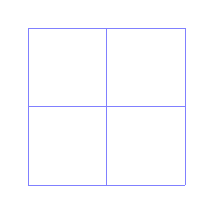
\begin{tikzpicture}[help lines/.style={blue!50,very thin}]
    \draw[help lines] (2,0) grid +(2,2);
  \end{tikzpicture}
\end{lstlisting}

\subsection{Path}
Add \texttt{-- cycle} at the end of a path will complete the path by
connecting back to the start.

\texttt{/tikz/every path} can be used to customize all path.

Operations
\begin{description}
\item [move-to] just coordinates
\item [line-to]
  \begin{description}
  \item [straight line] \texttt{-- (1,1)}
  \item [horizontal and vertical] \texttt{|-} or \texttt{-|}
  \end{description}
\item [curve-to] \texttt{.. controls <c> (and <d>) ..}
\item [rectangle] \texttt{(0,0) rectangle (1,1)}
\item [rounded corners]
\item [sharp corners]
\item [circle] \texttt{circle[⟨options⟩]}. It has option
  \texttt{/tikz/every circle}
  \begin{description}
  \item [x radius]
  \item [y radius]
  \item [radius]
  \item [at]
  \end{description}
\item [ellipse] ellipse[⟨options⟩] Same as circle
\item [arc]
  \begin{description}
  \item [start angle]
  \item [end angle]
  \item [delta angle]
  \end{description}
\item [grid] \verb$\draw[grid] (-2,0) grid (2,12);$
  \begin{description}
  \item [step]
  \item [xstep]
  \item [ystep]
  \item [help lines]
  \end{description}
\item [to] TODO
\item [foreach] TODO
\item [let] TODO
\end{description}

\subsection{Action}
\verb$\draw$ equals \verb$\path{draw}$
Action
\begin{description}
\item [draw]
\item [fill]
\item [filldraw]
\item [pattern] options: \texttt{pattern color}
  \begin{description}
  \item [dots]
  \item [fivepointed stars]
  \item [bricks]
  \end{description}
\item [shade] It has an option \texttt{shading
    angle=<degrees>}. Another option \texttt{shading=<name>} can be:
  \begin{description}
  \item [axis]
  \item [radial]
  \item [ball]
  \end{description}
\item [shadedraw]
\item [clip]
\item [useasboundingbox]
\end{description}


Graphic parameters
\begin{description}
\item [color] used for fill, draw, text. Can use \texttt{red!20!black}
  thanks to \texttt{color} package.
  \begin{description}
  \item [draw=<color>]
  \item [fill=<color>]
  \item [text=<color>] apply on text
  \end{description}

\item [draw] 
\item [line width] Line can be: ultra thin, very thin, thin,
  semithick, thick, very thick, ultra thick. Of course the more
  flexible way is using \texttt{line width = <dimension>}.
\item [dash patterns]
  \begin{description}
  \item [dash pattern=]
  \item [dash phase=]
  \item [solid]
  \item [<densely> <loosely> dotted]
  \item [<densely> <loosely> dashed]
  \item [<densely> <loosely> dash dot]
  \item [<densely> <loosely> dash dot dot]
  \end{description}
\item [double] with option \texttt{double distance=<dimension>}
\end{description}

\subsection{Arrows}
To add the arrow tips, first add \texttt{[->]} option for the tikz
environment.  The library \texttt{arrows.meta} defines etras arrow
types.


\subsection{Node \& Edge}

\begin{lstlisting}
node [⟨options⟩] (⟨name⟩) at (⟨coordinate⟩) {⟨contents⟩};
\end{lstlisting}

\verb$\path node$ equals \verb$\node$. \texttt{every node} and
\texttt{every <shape> node} is available.

Multi part node:
\begin{lstlisting}
  \node[circle split,draw,double,fill=red!20] {top \nodepart{lower} bot};
\end{lstlisting}

\subsubsection{Option}
\begin{description}
\item [align=left] have to have this to make the \verb$\\$ able to create
  newline
\item [shape=<shape name>] \texttt{shape=} is optional. Can be
  rectangle, circle.
\item [inner sep=<dimension>]
\item [inner xsep]
\item [inner ysep]
\item [outer sep]
\item [outer xsep]
\item [outer ysep]
\item [minimum height]
\item [minimum width]
\item [minimum size]
\end{description}


\subsubsection{Position}
\begin{description}
\item [anchor]
\item [above=<offset]
\item [below]
\item [left]
\item [right]
\item [above left]
\item [above right]
\item [below left]
\item [below right]
\item [centered]
\item [fit] \texttt{fit=(a) (b) (c)}
\end{description}

Placing node on edge
\begin{description}
\item [pos=<fraction>]
\item [auto]
\item [swap]
\item ['] alias of swap
\item [sloped]
\item [allow upside down]
\item [midway]
\item [near start] 0.25
\item [near end] 0.75
\item [very near start] 0.125
\item [very near end] 0.875
\item [at start]
\item [at end]
\end{description}

\subsubsection{Label \& Pin}
General syntax is \texttt{label=[<options>]<angle>:<text>}.
\texttt{every label/.style} is available.

Options:
\begin{description}
\item [label position=<angle>]
\item [absolute=boolean]
\item [label distance]
\end{description}

General syntax for pin is \texttt{pin=[<options>]<angle>:<text>}

options:
\begin{description}
\item [pin distance]
\item [every pin]
\item [pin position=<angle>]
\item [every pin edge]
\end{description}

The \texttt{quotes} package provides quote syntax:
\texttt{"<text>"<options>}. The option \texttt{every label quotes} is
available.
\begin{lstlisting}
\tikz \node ["my label" red, draw] {my node};
\end{lstlisting}


\subsection{Graph}
This requires the \texttt{graphs} library.

\begin{description}
\item [graph syntax] \verb$\path graph[⟨options⟩]⟨group specification⟩$
\item [group spec] \verb${[⟨options⟩]⟨list of chain specifications⟩}$
  The nodes can be grouped by surround them with curly braces. The
  entry and exit points are computed for the chains in and out the
  group.

\item [chain spec] consists of list of node spec seperated by edge
  spec
\item [edge spec] each accept an optional \texttt{[<options>]} after them.
  \begin{description}
  \item [->] directed edge
  \item [--] undirected edge
  \item [<-] backward
  \item [<->] bidirected
  \item [-!-] no edge
  \end{description}
\item [node spec] \verb$"<node name>"/"<text>"[<options>]$ The nodes
  used have a special notation. The quotes are required only when the
  node name contains special symbols. If the node name is empty, it
  will be given a random name.
\end{description}

Options
\begin{description}
\item [grow up/down/left/right]
\item [branch up/down/left/right]
\item [grow up/down/right/left sep=<distance>]
\item [branch up/down/left/right sep=<distance>]
\item [/tikz/graph/level <level>] \texttt{level 1/.style={}}
\end{description}

\subsection{Matrix}
The columns are separated by \verb$&$, rows by \verb$\\$. The last
line also needs an \verb$\\$.
\verb$\matrix$ equals to \verb$\path \node [matrix]$
\begin{lstlisting}
  \matrix {
    \node(a) {A}; & \node (b) {B}; \\
    \node(c) {C}; & \node (d) {D}; \\
  };
\end{lstlisting}

options
\begin{description}
\item [column sep]
\item [row sep]
\end{description}

option group
\begin{description}
\item [row/column <number>]
\item [row <number> column <number>]
\item [every odd/even row/column]
\end{description}


\subsection{Tree}

\begin{lstlisting}
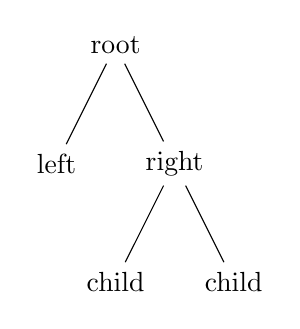
\begin{tikzpicture}
  \node {root}
    child {node {left}}
    child {node {right}
      child {node {child}}
      child {node {child}}
    };
\end{tikzpicture}
\end{lstlisting}

option
\begin{description}
\item [level distance]
\item [grow=<direction>]
\item [grow'=<direction>]
\end{description}

option group
\begin{description}
\item [level <number>]
\end{description}

\subsection{Decoration}
Must have \texttt{decorate} option, then specify the pattern by
\texttt{decoration=}. \texttt{random steps} is useful.

\begin{lstlisting}
decorate, decoration={random steps,segment length=3pt,amplitude=1pt}
\end{lstlisting}


\subsection{Package}
\subsubsection{shapes.multipart}
\begin{lstlisting}
mynode/.style={split, rectangle split parts=2}
\end{lstlisting}
\begin{description}
\item [patterns]
\item [positioning,fit,calc]
\item [decorations.pathmorphing]
\item [decorations.pathreplacing]
\item [quotes]
\item [graphs]
\item [arrows.meta]
\end{description}





%%% Local Variables:
%%% TeX-master: "cheatsheet"
%%% End:

\clearpage
\section{Prolog}

online resources
\begin{itemize}
\item learn prolog now \footnote{http://lpn.swi-prolog.org/lpnpage.php?pageid=top}
\item swipl library \footnote{http://www.swi-prolog.org/pldoc/man?section=lists}
\end{itemize}

\subsection{Running program}

Install swi-prolog, and emacs should be able to support it.  In a
prolog file, select a region, and \texttt{C-c C-c r} (execute region).
Using this for facts and rules, but evalute query direct in the repl.

\subsection{Concepts}

A Horn Clause: $c \quad h_1 \wedge h_2 \wedge \ldots \wedge h_n$.
$c$ is the consequent, the conjunction of $h_i$ is the antecedent.
It means if all $h_i$ are true, $c$ is true.
This is written in prolog as:

\begin{lstlisting}
  c :- h1,h2,...,hn
\end{lstlisting}

Logic program is actually a collection of Horn Clauses.
A logic problem has three components:
\begin{description}
\item [fact] Horn Clause with no Antecedent. isamother(mary)
\item [rule] Horn Clause with Antecendent
\item [query] Horn Clause with no Consequent
\end{description}

Example:

\begin{lstlisting}[language=prolog]
  % facts
  isamother(mary).
  childof(tom, mary).
  % rules
  loves(mary, tom) :- isamother(mary), childof(tom, mary).
  % quries
  ?- loves(mary, tom).
\end{lstlisting}

Prolog can have variables. Everything start from upper case letter or
underscore is a variable. A single underscore is anonymous
variable. Variables are often used in rules and quries.
\begin{lstlisting}
  loves(X, Y) :- isamother(X), childof(Y, X).
  ?- loves(mary, X).
\end{lstlisting}

Syntax of prolog:
\begin{lstlisting}
  Clause :: Predicate. | Predicate :- PredicateSeq.
  PredicateSeq :: Predicate | Predicate, PredicateSeq
  Predicate :: PredName(TermSeq)
  TermSeq :: Term | Term, TermSeq
  Term :: FunctorName(TermSeq) | Constant | Variable
\end{lstlisting}

\subsection{Executing}
\subsubsection{Unification}
Given two atomic formula (predicates), they can be unified if and only
if they can be made syntactically identical by replacing the variables
in them by some terms. For example, unify \texttt{childof(jane, X)}
and \texttt{childof(jane, mary)}.  \textit{MGU} results from a
substitution that bounds free variables as little as possible

\subsubsection{Substitution}
Substitution maps variables to terms.  Instantiation is the
application of substitution to all variables in a prolog formula,
term. E.g. unify $childof(jane, X)$ and $childof(Y, mary)$ by
$[X \rightarrow mary, Y \rightarrow jane]$

\subsubsection{Unification and Computing with Logic}

Given a query
\begin{itemize}
\item Search the facts and rules to find whether the query unifies
  with any consequent
\item If the search fails, return false (query result)
\item If the search is successful, then
  \begin{itemize}
  \item if the unification occurs with the consequent of a fact,
    return the substitution of the variables (if any)
  \item if the unification occurs with the consequent of a fact,
    return the substitution of the variables (if any)
  \end{itemize}
\end{itemize}

An example:
\begin{lstlisting}
isamother(mary).
childof(tom, mary).
loves(X, Y) :- isamother(X), childof(Y, X).
?- loves(mary, tom).
\end{lstlisting}

\subsubsection{Backtracking}

\begin{itemize}
\item Re-try to unify with some clause other than the fact, and proceed
\item Re-try to unify with some clause other than the fact, and proceed
\end{itemize}

Example:
\begin{lstlisting}
isamother(mary).
childof(jane, mary).
childof(tom, mary).
loves(X, Y) :- isamother(X), childof(Y, X).
?- loves(mary, X)
\end{lstlisting}

\subsection{Other Prolog Features}
\subsubsection{List}

\begin{itemize}
\item \texttt{[a, b, c]}: a list of 3 elements
\item \texttt{[]}: empty list
\item \texttt{[a, [b, c], [[d, e]], []]}: list can contain different type
\item \texttt{[a|[b, c]]}: head and tail
\end{itemize}

Example:
\begin{lstlisting}
  ?- [1, 2, 3] = [X|Xs].
  % X=1
  % Xs = [2, 3]
  ?- [1, 2, 3] = [X|[Y|Rest]].
  % X=1
  % Y=2
  % Rest = [3]
\end{lstlisting}

\subsubsection{if-then-else}
\begin{lstlisting}
  ?- Z = 3, (Z == 3 -> X = 1, Y = 2; X = 2, Y = 1).
  % Z=3
  % X=1
  % Y=2
\end{lstlisting}

\subsection{Examples}
\begin{lstlisting}
lectures(monday, nolecture).
lectures(tuesday, vp).
lectures(tuesday, se).
lectures(tuesday, ddbms).
lectures(wednessday, ds).
lectures(wednessday, mpl).
lectures(thursday, vp).
lectures(thrusday, se).
lectures(friday, ds).
lectures(friday, mpl).
lectures(saturday, ai).
lectures(saturday, ddbms).
%% ?- lectures(friday, X), write(X),nl.
%% ?- lectures(friday, X), write(X), nl, fail.
\end{lstlisting}

An graph example:
\begin{lstlisting}
edge(a, b).
edge(b, c).
edge(c, a).
reach(X, Y) :- edge(X, Y).
reach(X, Y) :- edge(X, Z), reach(Z, Y).
?- reach(a, c)
\end{lstlisting}



%%% Local Variables:
%%% TeX-master: "cheatsheet"
%%% End:

\clearpage
\section{AI}

\subsection{Agent Concept}

I'll give some questions in the homework ..

\begin{quote}
  An agent that senses only partial information about the state cannot
  be perfectly rational.
\end{quote}

False. The vacuum-cleaning agent is perfectly rational, but it senses
only partial information, i.e. it doesn't observe the state of the
square that is adjacent to it.

\begin{quote}
  There exist task environment in which no pure reflex agent can
  behave rationally.
\end{quote}
True. Purely reflective behavior does not take the percept history
into account, only the most recent percepts.

\begin{quote}
  There exists a task environment in which every agent is rational.
\end{quote}
True.  A task environment in which there are no decisions to be made:
all actions will receive the same output.

\begin{quote}
  The input to an agent program is the same as the input to the agent
  function
\end{quote}
False. The input to agent program: current percept while the input to
agent function: entire precept history.

\begin{quote}
  Every agent function is implementable by some program/machine
  combination
\end{quote}
False. As the textbook said: "No machine can tell /in general/ whether
a given program will return an answer on a given input or run
forever."

\begin{quote}
  suppose an agent selects its action uniformly at random from the set
  of possible actions.  There exists a deterministic task environment
  in which this agent is rational.
\end{quote}
True.  In the environment that all actions will produce same output,
it is rational.  Actually all agents are rational in such environment.

\begin{quote}
It is possible for a given agent to be perfectly rational in two distinct task environments.
\end{quote}

True.  There's recently a kickstarter project that produces dice with
more than 6 faces.  If an agent is rational in a N face dice bet game,
it will perform equally well in a 6-face dice or a 8-face dice.
\begin{quote}
Every agent is rational in an un-observable environment.
\end{quote}
False.  A vacuum agent that can move will be rational, but the one
that does not move is not.

\begin{quote}
A perfectly rational poker-playing agent never loses.
\end{quote}
False.  Two such perfectly rational agent play against each other will
give one lose.
      
\subsubsection{Agent function v.s. Agent program}
\begin{quote}
Can there be more than one agent program that implements a given agent
function? Give an example, or show why one is not possible.
\end{quote}
There are infinite agent programs that implement a given agent
function.  If an agent function acts only depend on previous $n$
percepts.  Than, the agent implementations that have n or more memory
will always produce the same action.

\begin{quote}
Are there agent functions that cannot be implemented by any agent program?
\end{quote}

Yes. As the textbook said: "No machine can tell /in general/ whether a
given program will return an answer on a given input or run forever."

\begin{quote}
  Given a fixed machine architecture, does each agent program
  implement exactly one agent function?
\end{quote}

Yes. A program implements a mapping from percepts to actions.  The
same percept will only result in one action.

\begin{quote}
  Given an architecture with n bits of storage, how many different
  possible agent programs are there?
\end{quote}

There would be $a^{2^n}$ possible programs; $2^n$ possible states and
$a$ choices for each state.

\begin{quote}
  Suppose we keep the a gent program fixed but speed up the machine by
  a factor of two. Does that change the agent function?
\end{quote}

No. The speed does not have influence on the produced action.






\subsection{State changing and implementation}
\subsubsection{hanoon jugs}
\begin{quote}
  Give a complete problem formulation for each of the following.
  Choose a formulation that is precise enough to be implemented.
  d. You have three jugs, measuring 12 gallons, 8 gallons, and 3 gallons, and a water faucet.
  You can fill the jugs up or empty them out from one to another or onto the ground.
  You need to measure out exactly one gallon.
\end{quote}

Define a 3-tuple =(x,y,z)= where x,y,z are the amount of water in the
three jugs.
\begin{itemize}
\item Initial state: =(0,0,0)=.
\item Action:
  \begin{itemize}
  \item FILL: given values =(x,y,z)= , generate =(12,y,z)=, =(x,8,z)=,
    =(x,y,4)=
  \item EMPTY: given values =(x,y,z)= , generate =(0,y,z)=, =(x,0,z)=,
    =(x,y,0)=
  \item POUR: Given value =(x,y)=, let ~t = min(x+y, cap(y))~, pour x
    into y, generate: =(x-(t-y), t)=
  \end{itemize}
\item Cost function: Number of actions.
\end{itemize}

\subsubsection{野人与传教士}
三个野人,三个传教士,一艘船。如何过河?


\paragraph{Formulate}
\begin{quote}
  Formulate the problem precisely. making only those distinctions
  necessary to ensure a valid solution. Draw a diagram of the complete
  state space.
\end{quote}

state
\begin{itemize}
\item =(M1,C1,B1,M2,C2,B2)= where =M1,C1,B1= is the number of missionaries, cannibals, boats on the left side,
  =(M2,C2,B2)= is the corresponding number on the right side.
\item The start state is =(3,3,1,0,0,0)=.
\item The goal: =(0,0,0,3,3,1)=
\end{itemize}
Action: =(m,c,b)= on left side: where b means the change of boat, m
and c means the change of missionaries and cannibals.  The action
allows the boat number B1 or B2 to change from 1 to 0, along with M
and C on the side move to the other side by one or two.
     
\begin{lstlisting}
  (-1 0 -1)
  (0 -1 -1)
  (-2 0 -1)
  (0 -2 -1)
  (-1 -1 -1)

  (1 0 1)
  (0 1 1)
  (2 0 1)
  (0 2 1)
  (1 1 1)
\end{lstlisting}
The complete state space.

In the table below, the striped items are those that cannibals will
eat missionaries.  The state that is not reachable
(e.g. =(3,3,0,0,0,1)=) is not striped out.

\begin{lstlisting}
| =(3 3 1 0 0 0)= | +=(3 2 1 0 1 0)=+ | +=(3 1 1 0 2 0)=+ | +=(3 0 1 0 3 0)=+  |
| +=(2 3 1 1 0 0)=+ | =(2 2 1 1 1 0)= | +=(2 1 1 1 2 0)=+ | +=(2 0 1 1 3 0)=+  |
| +=(1 3 1 2 0 0)=+ | +=(1 2 1 2 1 0)=+ | =(1 1 1 2 2 0)= | +=(1 0 1 2 3 0)=+  |
| +=(0 3 1 3 0 0)=+ | +=(0 2 1 3 1 0)=+ | +=(0 1 1 3 2 0)=+ | =(0 0 1 3 3 0)=  |
| =(3 3 0 0 0 1)= | +=(3 2 0 0 1 1)=+ | +=(3 1 0 0 2 1)=+ | +=(3 0 0 0 3 1)=+  |
| +=(2 3 0 1 0 1)=+ | =(2 2 0 1 1 1)= | +=(2 1 0 1 2 1)=+ | +=(2 0 0 1 3 1)=+  |
| +=(1 3 0 2 0 1)=+ | +=(1 2 0 2 1 1)=+ | =(1 1 0 2 2 1)= | +=(1 0 0 2 3 1)=+  |
| +=(0 3 0 3 0 1)=+ | +=(0 2 0 3 1 1)=+ | +=(0 1 0 3 2 1)=+ | =(0 0 0 3 3 1)=  |
\end{lstlisting}

\paragraph{Solve}
\begin{quote}
Implement and solve the problem optimally using an appropriate search algorithm.
Is it a good idea to check for repeated states?
\end{quote}

The solution:
\begin{lstlisting}
  (3,3,1,0,0,0)
  -> (2,2,0,1,1,1)
  -> (3,2,1,0,1,0)
  -> (3,0,0,0,3,1)
  -> (3,1,1,0,2,0)
  -> (1,1,0,2,2,1)
  -> (2,2,1,1,1,0)
  -> (0,2,0,3,1,1)
  -> (0,3,1,3,0,0)
  -> (0,1,0,3,2,1)
  -> (0,2,1,3,1,0)
  -> (0,0,0,3,1,0)
\end{lstlisting}
Yes, we should check repeated states to avoid infinite recursion.

\paragraph{discussion}
\begin{quote}
  Why do you think people have a hard time solving this puzzle,
  given that the state space is so simple?
\end{quote}

\begin{enumerate}
\item It is hard to manually work it out.
\item the repeat states need to be removed, which increase difficulty for manual solving.
\end{enumerate}



\subsection{Search Algorithm}

\subsubsection{branching factor, BFS, DFS}
\begin{quote}
  3.26 Consider the unbounded version of regular 2D grid shown in Figure 39.
  The start state is at the origin, (0,0), and the goal state is at (x,y).
\end{quote}

\begin{itemize}
\item What is the branching factor b in the state space?
  \begin{itemize}
  \item Since it is a 2D grid, there're 4 directions for each node. The branching factor is 4.
  \end{itemize}
\item How many distict states are there at depth k (for k > 0)?
  \begin{itemize}
  \item For depth 1, there're 1+4 states;
  \item For depth 2, there're 1+4+8 states;
  \item For depth 3, there're 1+4+8+12 states;
  \item For depth k, there're $1 + 4 + 8 + .. + 4k = 2k^2 + 2k + 1$
  \end{itemize}
\item What is the maximum number of nodes expanded by breadth-first
  tree search?
  \begin{itemize}
  \item The depth of the goal is |x|+|y|, and if we allow the loopy
    states on the search tree, we will have 4 branches for each
    node. Thus the maximum total nodes to be expanded:
    $1 + 4^1 + 4^2 + .. + 4^(|x|+|y|)$
  \end{itemize}
\item What is the maximum number of nodes expanded by breadth-first
  graph search?
  \begin{itemize}
  \item For graph search, we only expand nodes that are not in
    exploded set.  The expanded nodes will be the distinct state of
    depth |x|+|y|: 1 + 4 + 8 + .. + 4k
  \end{itemize}
\item Is h= |u-x| + |v-y| an admissible heuristic for a state at
  (u,v)? explain.
  \begin{itemize}
  \item Yes. Because it never overestimates the cost: it is the
    optimal path from (u,v) to (x,y) in a 2D grid given that all links
    cost 1.
  \end{itemize}
\item How many nodes are expanded by A* graph search using h?
  \begin{itemize}
  \item It is |x|*|y|. Because all the paths in the rectangle are
    optimal paths.
  \end{itemize}
\item Does h remain admissible if some links are removed?
  \begin{itemize}
  \item Yes. Removing links can only make the best path longer if
    possible, so h remains an underestimate.
  \end{itemize}
\item Does h remain admissible if some links are added between
  nonadjacent states?
  \begin{itemize}
  \item No. We could add some links that makes the optimal solution
    shorter.  Thus h would overestimate the cost.
  \end{itemize}
\end{itemize}


\subsection{Formulation}
\subsubsection{Floor planning}
\begin{quote}
6.4 Given the precise formulations for each of the following as a Constraint Satisfaction Problems:
Rectilinear floor-planning: find non-overlapping places in a large rectangle for a number of smaller rectangles.
\end{quote}

\begin{description}
\item [Variables]
  \begin{itemize}
  \item WIDTH and HEIGHT for the large rectangle.
  \item $R_i$ for each rectangles, $R_{i}$.w and $R_{i}.h$ for the width and height of $R_i$ respectively.
  \item the position $P_i$ for \textit{top-left} corner of the rectangle $R_i (P_{i}.x$ and $P_{i}.y$ for the co-ordinates)
  \end{itemize}
\item [Domains] ${P_{i}.x \in [0, WIDTH]}$
\item [Constraints] the four corners of $R_i$ should not be inside the
  area of $R_j$, for each $i \neq j$
  \begin{itemize}
  \item  for each $i \neq j$
  \item  for each corner $(x,y)$ in
    $\{(P_{i}.x, P_{i}.y)$, $(P_i.x + R_i.w, P_i.y)$, $(P_i.x, P_i.y + R_i.h)$, $(P_i.x+R_i.w, P_i.y + R_i.h)\}$
  \item  $\neg (P_{j}.x < x < P_{j}.x + R_{j}.w \cap P_{j}.y < y < P_{j}.y + R_{j}.h)$
  \end{itemize}
\end{description}

\subsubsection{class scheduling}
\begin{quote}
  Class scheduling: There is a fixed number of professors and
  classrooms, a list of classes to be offered, and a list of possible
  time slots for classes.  Each professor has a set of classes that he
  or she can teach.
\end{quote}

\begin{description}
\item [Variables]
  \begin{itemize}
  \item $P_i$ for each professor, with $P_i.classes$ be the set of classes he or she can teach
  \item $R_i$ for each room
  \item $C_i$ for each class
  \item $T_i$ for each time slot
  \item Assignment $A_i$, the i-th assignment, is a 4-tuple $(A_i.prof, A_i.room, A_i.class, A_i.time)$.
  \end{itemize}
\item [Domain]
  \begin{itemize}
  \item $A_i.prof \in {P_j}$
  \item $A_i.room \in {R_j}$
  \item $A_i.class \in {C_j}$
  \item $A_i.time \in {T_j}$
  \end{itemize}
\item [Constraint]
  \begin{itemize}
  \item $A_i.class \in A_i.prof.classes$ for all i
  \item $\neg (A_i.time = A_j.time \cap A_i.prof = A_j.prof)$ for all $i \neq j$
  \item $\neg (A_i.time = A_j.time \cap A_i.room = A_j.room)$ for all $i \neq j$
  \end{itemize}
\end{description}


\subsubsection{linving in 5 houses}
\begin{quote}
  Consider the following logic puzzle: In five houses, each with a
  different color, live five persons of different nationalities, each
  of whom prefers a different brand of candy, a different drink, and a
  different pet.  Given the following facts, the questions to answer
  are "where does the zebra live, and in which house do they drink
  water?"  Discuss different representations of this problem as a CSP.
  Why would one prefer one representation over another?
  \begin{itemize}
  \item The Englishman lives in the red house.
  \item The Spaniard owns the dog.
  \item The Norwegian lives in the first house on the left.
  \item The green house is immediately to the right of the ivory house.
  \item The man who eats Hershey bars lives in the house next to the man with the fox.
  \item Kit Kats are eaten in the yellow house.
  \item The Norwegian lives next to the blue house.
  \item The Smarties eater owns snails.
  \item The Snickers eater drinks orange juice.
  \item The Ukrainian drinks tea.
  \item The Japanese eats Milky Ways.
  \item Kit Kats are eaten in a house next to the house where the horse is kept.
  \item Coffee is drunk in the green house.
  \item Milk is drunk in the middle house.
  \end{itemize}
\end{quote}


\paragraph{First representation}
This representation is based on the house.
\begin{description}
\item [Variables and domains] H for the houses
  \begin{description}
  \item [.n] nationality
  \item [.b] hold brand of candy
  \item [.lb] the one lived in this house like the brand of candy
  \item [.c] color
  \item [.d] hold drink
  \item [.ld] the man lived in this house like the drink
  \item [.pet] hold pet
  \item [.index] index of the house from left to right
  \end{description}
\item [Domains]
  \begin{itemize}
  \item h.n $\in$ Englishman, Spaniard, etc.
  \item h.c $\in$ red, green, etc.
  \item h.b $\in$ ivory, smarties, etc.
  \item h.d $\in$ water, tea, etc.
  \item h.p $\in$ dog, fox, snail, etc.
  \item h.index $\in$ [1,5]
\end{itemize}
\item [Constraints]
  \begin{itemize}
  \item The Englishman lives in the red house. \\
    $\neg h.c=red \cup h.n=Englishman$
  \item The Spaniard owns the dog. \\
    $\neg h.n=Spanisard \cup h.pet=dog$
  \item The Norwegian lives in the first house on the left.\\
    $\neg h.n = Norwegian \cup h.index = 1$
  \item The green house is immediately to the right of the ivory house.\\
    $\neg (h1.c = green \cap h2.b = ivory) \cup h1.index = h2.index + 1$
  \item The man who eats Hershey bars lives in the house next to the man with the fox.\\
    $\neg (h1.lb=Hersheybar \cap \cap h2.pet = fox) \cup | h1.index-h2.index | = 1$
  \item Kit Kats are eaten in the yellow house.\\
    $\neg h.c=yellow \cup h.lb = KitKats$
  \item The Norwegian lives next to the blue house.\\
    $\neg (h1.n=Norwegian \cap h2.c = blue) \cup | h1.index - h2.index |=1$
  \item The Smarties eater owns snails.\\
    $\neg h.lb=smarties \cup h.p = snails$
  \item The Snickers eater drinks orange juice.\\
    $\neg h.lb=snickers \cup h.ld = OrangeJuice$
  \item The Ukrainian drinks tea.
    $\neg h.n=Ukrainian \cup h.ld=tea$
  \item The Japanese eats Milky Ways.
    $\neg h.n=Japanese \cup h.lb=MilkyWays$
  \item Kit Kats are eaten in a house next to the house where the horse is kept.
    $\neg (h1.b=Kats \cap h2.pet=horse) \cup |h1.index-h2.index|=1$
  \item Coffee is drunk in the green house.
    $\neg h.d=coffee \cup h.c=green$
  \item Milk is drunk in the middle house.
    $\neg h.d=milk \cup h.index=3$
  \end{itemize}
\end{description}

\paragraph{Second Representation}
This representation is based on the Person.  The domains and
constraints are similar.

\begin{description}
\item [Variables] P for person
  \begin{itemize}
  \item .n : nationality
  \item .b : in his house, the candy that holds
  \item .lb : the brand of candy he likes
  \item .c : the color of his house
  \item .d: the drink held in his house
  \item .ld: the drink he likes
  \item .pet: his pet
  \item .index: the index of his house
  \end{itemize}
  
\end{description}

    
\paragraph{Comparison}
Similarly, we can also derive the representation based on other
variables, e.g. drink, candy, etc.  One would prefer one to the other
based on the query type he want.  For example, if the query is based
on the house, e.g. which house hold some drink, he would prefer the
house-based representation.  Similarly if the query is based on
person, e.g. what pet does the Englishman keeps, he would prefer the
person-based representation.  But essentially they are the same.



\subsection{Propositional Logic}
\subsubsection{Simple}
\begin{quote}
  Given the following, can you prove that the unicorn is mythical?
  How about magical? Horned?

  If the unicorn is mythical, then it is immortal,
  but if it is not mythical, then it is a mortal mammal.
  If the unicorn is either immortal or a mammal, then it is horned.
  The unicorn is magical if it is horned.
\end{quote}

The formula writes:
\begin{itemize}
\item $\neg mythical \vee immortal$
\item $mythical \vee mammal$
\item $\neg (immortal \vee mammal) \vee horned$
\item $\neg horned \vee magical$
\end{itemize}

We have the enumerated truth table:
\begin{lstlisting}
| mythical | immortal | mammal | horned | magical |
|----------+----------+--------+--------+---------|
| T        | T        | T      | T      | T       |
| T        | T        | F      | T      | T       |
| F        | T        | T      | T      | T       |
| F        | F        | T      | T      | T       |
\end{lstlisting}

Based on these, we can derive:
\begin{itemize}
\item We cannot prove unicorn is mythical.
\item We can prove it is magical.
\item We can prove it is horned.
\end{itemize}

\subsubsection{Party resolution}
\begin{quote}
  7.18 Consider the following sentence:
  $$
  ((Food \Rightarrow Party) \vee (Drinks \Rightarrow Party))
  \Rightarrow ((food \wedge drinks) \Rightarrow Party)
  $$
  \begin{enumerate}
  \item Determine, use enumeration, whether the sentence is
    valid, satisfiable (but neg valid), or unsatisfiable.
  \item Convert the left-hand and right-hand sides of the main
    implication into CNF, Showing each step, and explain how the
    results confirm your answer to (a)
  \item Prove your answer to (a) using resolution.
  \end{enumerate}
\end{quote}

\paragraph{1}
It is Valid.
The enumeration:

\begin{tabular}{l|l|l|l|l|l}
  F & D & P & left hand & right hand & left $\Rightarrow$ right\\
  \hline
  T & T & T & T         & T          & T\\
  T & F & T & T         & T          & T\\
  F & T & T & T         & T          & T\\
  F & F & T & T         & T          & T\\
  \hline
  T & T & F & F         & F          & T\\
  T & F & F & T         & T          & T\\
  F & T & F & T         & T          & T\\
  F & F & F & T         & T          & T
\end{tabular}

\paragraph{2}
left-hand CNF:
\begin{eqnarray}
  ((F \Rightarrow P) \vee (D \Rightarrow P)\\
  \spadesuit (\neg F \vee P) \vee (\neg D \vee P)\\
  \spadesuit (\neg F \vee P \vee \neg D \vee P)\\
  \spadesuit (\neg F \vee \neg D \vee P)\\
\end{eqnarray}

right-hand CNF:
\begin{eqnarray}
  (F \wedge D) \Rightarrow P\\
  \spadesuit \neg (F \wedge D) \vee P\\
  \spadesuit (\neg F \vee \neg D) \vee P\\
  \spadesuit \neg F \vee \neg D \vee P
\end{eqnarray}

As we can see, they are exactly the same. Thus the production is valid.

\paragraph{3}
We can prove it by proving the negation is unsatisfiable.

$$\neg ((F \Rightarrow P) \vee (D \Rightarrow P) \Rightarrow ((F \vee D) \Rightarrow P))$$

\begin{eqnarray}
  \spadesuit \neg (((F \Rightarrow P) \vee (D \Rightarrow P)) \Rightarrow ((F \wedge D) \Rightarrow P))\\
  \spadesuit \neg ( \neg ((F \Rightarrow P) \vee (D \Rightarrow P)) \vee ((F \wedge D) \Rightarrow P))\\
  \spadesuit ((F \Rightarrow P) \vee (D \Rightarrow P)) \wedge (\neg ((F \wedge D) \Rightarrow P))\\
  \spadesuit ((\neg F \vee P) \vee (\neg D \vee P)) \wedge (\neg (\neg (F \wedge D) \vee P))\\
  \spadesuit (\neg F \vee \neg D \vee P) \wedge (F \wedge D) \wedge \neg P\\
  \spadesuit (\neg F \vee \neg D \vee P) \wedge F \wedge D \wedge \neg P
\end{eqnarray}
This resolves to empty clause, thus the original sentence is valid.



\subsection{Adversarial Search}

This is multiple agents, also known as /game/.

\subsubsection{Minimax Algorithm}
There're two players, Min and Max, each takes turn to execute.  Max
moves first.

\subsubsection{The optimal strategies}

% \begin{equation*}
%   MINIMAX-VALUE(n) = \left\{
%   \begin{array}{r1}
%     Utility(n) & \text {if n is terminal},\\
%     max_{s \in succ(n)} MINIMAX-VALUE(s) & \text{if n is a max node},\\
%     min_{s \in succ(n)} MINIMAX-VALUE(s) & \text{if n is a min node}.
%   \end{array} \right .
% \end{equation*}

Basically it recursively solve the problem.  The Utility function is
the payoff.  It actually list the tree of state space, and it is
optimal.

\subsubsection{Alpha-Beta pruning}
The problem of minimax algorithm is its node grow exponential.  This
algorithm is used to prune the subtree that does not affect the
result.

This is similar for MiniMax algorithm
\begin{itemize}
\item $\alpha$ is the value of the best choise so far, for max, init
  from $-\infty$
\item $\beta$ is the best value for min, init from $+\infty$
\end{itemize}

There're two procedures:
\begin{description}
\item [Alpha-Beta-Search(state)] returns an action. state is the current state.
\item [Max-Value(state, $\alpha$, $\beta$)] returns a utility value
\item [Min-Value(state, $\alpha$, $\beta$)] returns a utility value
\end{description}

\begin{lstlisting}
Alpha-Beta-Search(state) {
  v = Max-Value(state, -999, +999);
  return action in ACTIONS with value v;
}
Max-Value(state, alpha, beta) {
  v = INT_MIN;
  for each a in ACTIONS(state) do
    v = Max(v, Min-Value(result(s,a), alpha, beta));
    if v >= beta then return v;
    alpha = MAX(alpha,v);
  return v;
}
\end{lstlisting}

\subsection{Constraint Satisfaction Problems}
It seems to formulate the search problems in a uniformed
representation:
\begin{description}
\item [X] a set of variables
\item [D] each has a domain of values
\item [C] a set of constraints for each of the variable
\end{description}

The goal is to find the assignment of values to the variables, that satisfies the constraints.

\subsubsection{Advantage}
it uses /general purpose heuristic/ rather than /problem-specific/ ones.

\subsubsection{Variations}
\begin{itemize}
\item continuous or discrete domain
\item finite or infinite domain
\item linear or non-linear constraint
\item unary or binary or high order constraint
\end{itemize}




\subsection{Logic}
\subsubsection[entailment]
Entailment: $\beta \models \alpha$, reads: the sentence $\beta$ entails
the sentence $\alpha$ if and only if $\alpha$ is true in all worlds where
$\beta$ is true.

\subsubsection{Propositional logic}
a.k.a. boolean logic.

logical equivalence;

\begin{tabular}{l|l}
  a                                   & b\\
  \hline
  $\alpha \wedge \beta$                 & $\beta \wedge \alpha$\\
  $(\alpha \wedge \beta) \wedge \gamma$ & $\alpha \wedge (\beta \wedge \gamma)$\\
  $\alpha \Rightarrow \beta$            & $\neg \beta \Rightarrow \neg \alpha$\\
  $\alpha \Rightarrow \beta$            & $\neg \alpha \vee \beta$\\
  $\alpha \Leftrightarrow \beta$        & $(\alpha \Rightarrow \beta) \wedge (\beta \Rightarrow \alpha)$
\end{tabular}

\begin{itemize}
\item A sentence is /valid/ if it is true in all models.
  Deduction theorem: $KB \models \alpha$ iff $KB \Rightarrow
  \alpha$ is valid
\item A sentence is satisfiable if it is true in /some/ models.
  $KB \models \alpha$ iff $KB \wedge \neg \alpha$ is unsatisfiable.
\end{itemize}

Proof method:
\begin{itemize}
\item inference rules: transform the sentences to a normal form
\item model checking: truth table
\end{itemize}

A clause is a disjunction of literals.
Factoring: the result clause keeps only one copy of each literal.

Conjunction: $\wedge$
Disjunction: $\vee$
CNF: conjunctive normal form. Conjunction of (disjunctions of literals).


Resolution algorithm: proof by contradiction.
I.e. to show $KB \models \alpha$, we show $KB \wedge \neg \alpha$ is unsatisfiable.
The naming resolution is because, the pair of complementary literals is resolved.

Definite clause: disjunction of literals with exactly one positive literal.


\subsubsection{First Order Logic}
$\wedge$ is the natural connective with $\exists$.
Using $\Rightarrow$ as the main connective with $\exists$ often causes errors:

$$\exists x At(x,ISU) \Rightarrow Smart(x)$$

is true if there's anyone who is not at ISU, which may not be what you want.

Properties:
\begin{lstlisting}
  | a                   | b                   | result    |
  |---------------------+---------------------+-----------|
  | \forall x \forall y | \forall y \forall x |           |
  | \exists x \exists y | \exists y \exists x |           |
  | \exists x \forall y | \forall y \exists x | not equal |
  | \forall x           | \neg \exists x \neg |           |
  | \exists x           | \neg \forall x \neg |           |
\end{lstlisting}



\subsection{First order logic}
\subsubsection{Some problems}
\paragraph{Student problems}
\begin{quote}
  \begin{enumerate}
  \item /Some students took French in spring 2001./
  \item /Every student who takes French passes it./
  \item /Only one student took Greek in spring 2001./
  \item /The best score in Greek is always higher than the best score in French./
  \end{enumerate}
\end{quote}

\begin{description}
\item [student(x)] x is student
\item [f,g] French and German courses
\item [take(x,c,s)] student =x= takes course =c= in semester =s=
\item [pass(x,c)] student =x= passes course =c=
\item [score(x,c,s)] the score of student =x= in course =c= in semester =s=.
\item [x>y] x is greater than y
\end{description}

\begin{quote}
  \begin{enumerate}
  \item $\exists x student(x) \wedge take(x,f,spring2001)$
  \item $\forall x,s student(s) \wedge take(x,f,s) \Rightarrow pass(x,f,s)$
  \item $\exists x student(x) \wedge take(x,g,sprint2001) \wedge \forall \: y y \ne x \Rightarrow \neg take(y,g,sprint2001)$
  \item $\forall s \exists x \forall y score(x,g,s) > score(y,f,s)$
  \end{enumerate}
\end{quote}

\paragraph{pollicy problems}

\begin{quote}
    5. /Every person who buys a policy is smart./
    6. /No person buys an expensive policy./
    7. /There is an agent who sells policies only to people who are not insured./
\end{quote}

\begin{description}
\item [person(x)] x is person
\item [expensive(x)] x is expensive
\item [agent(x)] x is agent
\item [insured(x)] x is insured
\item [smart(x)] x is smart
\item [buy(x,y,z)] =x= buys =y= from =z=
\item [sell(x,y,z)] =x= sells =y= to =z=
\end{description}

\begin{quote}
  \begin{enumerate}
  \item $\forall person(x) \wedge (\exists y,z policy(y) \wedge buy(x,y,z)) \Rightarrow smart(x)$
  \item $\forall x,y,z person(x) \wedge policy(y) \wedge expensive(y) \Rightarrow \neg buy(x,y,z)$
  \item $\exists x agent(x) \wedge \forall y,z policy(y) \wedge sell(x,y,z) \Rightarrow (person(z) \wedge \neg insured(z))$
  \end{enumerate}
\end{quote}

\paragraph{barber}
\begin{quote}
  8. /There is a barber who shaves all men in town who do not shave themselves./
\end{quote}
\begin{description}
\item [man(x)] x is man
\item [barber(x)] x is a barber
\item [shaves(x,y)] =x= shaves =y=
\end{description}
\begin{quote}
  8. $\exists x \forall y barber(x) \wedge man(y) \wedge \neg shaves(y,y) \Rightarrow shaves(x,y)$
\end{quote}


\paragraph{citizen}
\begin{quote}
    9. /A person born in the UK, each of whose parents is a UK citizen or a UK resident, is a UK citizen by birth./
    10. /A person born outside the UK, one of whose parents is a UK citizen by birth, is a UK citizen by descent./
\end{quote}
\begin{description}
\item [person(x)] x is person
\item [parent(x,y)] =x= is parent of =y=
\item [citizen(x,c)] =x= is a citizen of country =c=
\item [citizen(x,c,r)] =x= is a citizen of country =c=, for reason =r=
\item [resident(x,c)] =x= is a resident of country =c=
\item [born(x,c)] =x= was born in country =c=
\end{description}

\begin{quote}
  \begin{enumerate}
  \item
    $\forall x person(x) \wedge born(x,UK) \wedge (\forall y
    parent(y,x) \Rightarrow ((\exists r citizen(y,UK,r)) \vee
    resident(y,UK))) \Rightarrow citizen(x,UK,BIRTH)$
  \item
    $\forall x person(x) \wedge \neg born(x,UK) \wedge (\exists y
    parent(y,x) \wedge citizen(y,UK,BIRTH)) \Rightarrow
    citizen(x,UK,DESCENT)$
  \end{enumerate}
\end{quote}

\paragraph{other}
\begin{quote}
    11. /Politicians can fool some of the people all of the time,/
        /and they can fool all of the people some of the time,/
        /but they can’t fool all of the people all of the time./

    12. /All Greeks speak the same language. (Use Speaks(x,l) to mean that person x speaks language l.)/
\end{quote}
\begin{description}
\item [person(x)] x is person
\item [politician(x)] x is politician
\item [fool(x,y,t)] =x= fools =y= at time =t=
\item [german(x)] =x= is German.
\end{description}
\begin{quote}
  \begin{enumerate}
  \item
    $\forall x politician(x) \Rightarrow (\exists y \forall t
    person(y) \wedge fool(x,y,t)) \wedge (\exists t \forall y
    person(y) \Rightarrow fool(x,y,t)) \wedge \neg (\forall t \forall
    y person(y) \Rightarrow fool(x,y,t))$
  \item
    $\forall x,y,l german(x) \wedge german(y) \wedge Speaks(x,l)
    \Rightarrow Speaks(y,l)$
  \end{enumerate}
\end{quote}

\subsubsection{ Unify}
\begin{quote}
  /For each pair of atomic sentences, give the most general unifier if it exists:/
  \begin{enumerate}
  \item $P(A,B,B), P(x,y,z)$
  \item $Q(y,G(A,B)),Q(G(x,x),y)$
  \item $Older(Father(y),y),Older(Father(x),John)$
  \item $Knows(Father(y),y), Knows(x,x)$
  \end{enumerate}
\end{quote}

\paragraph{1} {x/A, y/B, z/B}

\begin{eqnarray}
    /P(A,B,B), P(x,y,z)/\\
    \Rightarrow /P(A,B,B), P(A,y,z)/ : {x/A}\\
    \Rightarrow /P(A,B,B), P(A,B,z)/ : {x/A, y/B}\\
    \Rightarrow /P(A,B,B), P(A,B,B)/ : {x/A, y/B, z/B}
\end{eqnarray}

\paragraph{2}
Cannot unify.
To see why:

\begin{eqnarray}
    Q(y,G(A,B)),Q(G(x,x),y) : {y/G(x,x)}\\
    \Rightarrow Q(G(x,x), G(A,B)), Q(G(x,x), G(x,x)) : {y/G(x,x), x/A}\\
    \Rightarrow Q(G(A,A), G(A,B)), Q(G(A,A), G(A,A))
\end{eqnarray}
In the last formula, A cannot be unified to B.

\paragraph{3}
{x/John, y/John}

\begin{eqnarray}
  /Older(Father(y),y),Older(Father(x),John)/\\
  \Rightarrow /Older(Father(John),John),Older(Father(x),John)/ : {y/John}\\
  \Rightarrow /Older(Father(John),John),Older(Father(John),John)/ : {y/John, x/John}
\end{eqnarray}

\paragraph{4}
cannot unify.
\begin{eqnarray}
  Knows(Father(y),y), Knows(x,x) : {x/Father(y)}\\
  \Rightarrow Knows(Father(y),y), Knows(Father(y),Father(y))
\end{eqnarray}

In the last formula, y cannot be unified to Father(y).

\subsubsection{Barber}
\begin{quote}
   /9.20 Let L be the first-order language with a single predicate S(p, q),/
   /meaning “p shaves q.” Assume a domain of people./

   \begin{enumerate}
   \item /Consider the sentence “There exists a person P who shaves every one who does not shave themselves,/
     /and only people that do not shave themselves.”/
     /Express this in L./
   \item /Convert the sentence in (a) to clausal form./
   \item /Construct a resolution proof to show that the clauses in (b) are inherently inconsistent./
     /(Note: you do not need any additional axioms.)/
   \end{enumerate}
\end{quote}

\paragraph{1}
$$\exists p \forall q person(p) \wedge person(q) \wedge (\neg S(q,q) \Leftrightarrow S(p,q))$$

\paragraph{2}
1st order formula:

\begin{equation}
  \exists p \: \forall q \: person(p) \wedge person(q) \wedge (\neg S(q,q) \Leftrightarrow S(p,q))
\end{equation}

\begin{equation}
  \exists p \: \forall q \: person(p) \wedge person(q) \wedge (\neg S(q,q) \Rightarrow S(p,q)) \wedge (S(p,q) \Rightarrow \neg S(q,q))
\end{equation}

remove implication:

\begin{equation}
  \exists p \: \forall q \: person(p) \wedge person(q) \wedge (S(q,q) \vee S(p,q)) \wedge (\neg S(p,q) \vee \neg S(q,q))
\end{equation}

skolemize off the existence:

\begin{equation}
  \forall q \: person(P) \wedge person(q) \wedge (S(q,q) \vee S(P,q)) \wedge (\neg S(P,q) \vee \neg S(q,q)) : \{p={P}\}
\end{equation}

drop universal qualifier:

\begin{equation}
  person(P) \wedge person(q) \wedge (S(q,q) \vee S(P,q)) \wedge (\neg S(P,q) \vee \neg S(q,q))
\end{equation}

\paragraph{3}

The CNF above resolves to empty clause, which is false, meaning the logic is not satisfiable.


\subsection{Bayesian}
\begin{itemize}
\item  Node X is conditionally independent of all other nodes in the
  network, given its markov blanket. (parents, children, and
  children's parents).
\item  Node X is conditionally independent of its non-descendants given its
  parent.
\end{itemize}

\begin{description}
\item [sample space] The set of all possible worlds
\item [$\Omega$] the sample space
\item [$\omega$] an element of the space. Each element has a probability
  $P(\omega)$, and sum up to one.
\item [prior] also called /unconditional probabilities/ or /prior
  probabilities/.
\item [posterior] also called /conditional probability/ or /posterior
  probability/.
\item [evidence] the results observed
\item [product rule] A different form of the definition of conditional probability
  $P(a\wedge b) = P(a|b) P(b)$
\item [random variables] begin with uppercase letter.
\item [domain] the set of possible values the random variable can take
\item [probability distribution] for discrete random variables
\item [probability density function] for continuous random variables,
  because the vector is infinite.
\item [joint probability distribution] the P for two variables with some
  interaction
\item [full joint probability distribution] all variables
\item [inclusion-exclusion principle]
  $P(a\vee b) = P(a) + P(b) - P(a\wedge b)$
\item [probabilistic inference] computation of posterior probabilities given evidence
\item [marginalization] also called /summing out/, because it sums the
  conditional probabilities. The process of computing the
  unconditional probability, aka marginal probability
\item [normalization] when calculating a conditional probability, there's
  a constant. It is typically not important, so replace it with
  $\alpha$. The alpha is to set the probabilities to sum to 1.
  $P(X|e) = \alpha P(X,e)$
\item [conditioning rule] $P(Y) = \sum_{z} P(Y|z)P(z)$
\item [(absolute) independence] $P(X|Y)=P(X)$
\item [Bayes rule] $P(b|a) = \frac{P(a|b)P(b)}{P(a)}$
\item [conditional independence] $P(X,Y|Z) = P(X|Z) P(Y|Z)$
\item [naive Bayes] a single cause directly influences a number of
  effects, all of which conditionally independent, given the cause.
  It is also called /Bayesian classifier/, /idiot Bayes/.
  $P(Cause,E1,E2,...,En) = P(Cause) \prod_i P(Ei|Cause)$
\item [conditional probability table (CPT)] each row shows a conditional probability
\item each variable is conditionally independent of its non-descendants, given its parents.
\item [Markov blanket] parents, children, and children's parents
\end{description}

For continuous variables, the Bayes needs to do something.  Of course
we can do discretization, but the precision is lost.  One common
solution is to define standard families of probability density
functions, with a finite number of parameters.
Another solution is non-parameter one.
Now I list some parameter models.

\begin{description}
\item [Gausion (normal) distribution] $N(\mu, \sigma^2)(x)$ has the mean $\mu$ and the variance $\sigma^2$.
\end{description}


A network with both discrete and continuous variables is called hybrid
Bayesian network.
\begin{description}
\item [linear Gaussian]
\item [conditional Gaussian]
\item [probit distribution]
\item [logit distribution]
\item [logistic function]
\end{description}

Exact Inference
\begin{description}
\item [query variables]
\item [event] some assignments to a set of evidence variables
\item [evidence variables]
\item [hidden variables] non-query non-evidence variables
\end{description}





%%% Local Variables:
%%% TeX-master: "cheatsheet"
%%% End:

\clearpage
\section{AWK}
\subsection{Usage}


In shell, awk can be invoked like below. MUST USE single quote.

\begin{lstlisting}
awk 'pattern {action}'
awk 'pattern {action}' input.txt
awk -f script.awk input.txt
\end{lstlisting}

The form is \verb$pattern {action}$
A missing action means print the line;
a missing pattern always matches.
Pattern-action statements are separated by newlines or semicolons.

\subsection{Variables}
\begin{description}
\item [FS] \textit{Field Separator}. regular expression used to
  separate fields; also settable by option \texttt{-Ffs}.
\item [NF] number of fields in the current record
\item [NR] ordinal number of the current record
\item [FNR] ordinal number of the current record in the current file
\item [FILENAME] the name of the current input file
\item [RS] input record separator (default newline)
\item [OFS] output field separator (default blank)
\item [ORS] output record separator (default newline)
\end{description}


\subsection{patterns}

Patterns are arbitrary Boolean combinations (with \verb$!$= \verb$||$ \verb$&&$)
of regular expressions and relational expressions.

A pattern may consist of two patterns separated by a comma; in this
case, the action is performed for all lines from an occurrence of the
first pattern though an occurrence of the second.

special patterns: \texttt{BEGIN}, \texttt{END}.
Cannot combine with other patterns.

\subsection{actions}

An action is a sequence of statements.
Statements are terminated by semicolons, newlines or right braces

\subsection{variable}
awk is line-based, and the content of lines are splited into fields
\texttt{\$1}, \texttt{\$2}, etc, by the separator \texttt{FS}.
\texttt{\$0} refers to the entire line.

\subsection{examples}

\begin{lstlisting}
awk 'NR==10 {print}' input.txt # output 10th line, or empty is less than 10 lines
\end{lstlisting}


%%% Local Variables:
%%% TeX-master: "cheatsheet"
%%% End:

\clearpage
\section{sed}

\subsection{Introduction}
The sed version on Mac OS and GNU Linux are different.
So, use gnu! On Mac, install
\begin{lstlisting}
brew install gnu-sed
\end{lstlisting}

This will make a =gsed= command available.
To write a cross platform script, use
\begin{lstlisting}
echo "OSTYPE: " $OSTYPE
SED=sed
if [[ "$OSTYPE" == "linux-gnu" ]]; then
    SED=sed
elif [[ "$OSTYPE" == "darwin"* ]]; then
    SED=gsed
fi
$SED -E -e "460,$ s/REG[0-9]{1,2}//g" compress42.c.orig > compress42.bugsig.c
\end{lstlisting}

\subsubsection{About the regular expression version}
\texttt{-E} will enable extra features, such as: \texttt{a{1,2}}
See \verb$re_format(7)$ for details.

There's no =\d=, so use =[0-9]= instead. The man page says =[:digit:]= can be used, but it seems not working.

\subsection{usage}
in shell script

\begin{lstlisting}
#!/bin/sed -f
#!/bin/sed -nf
\end{lstlisting}

\subsection{concepts}
\begin{description}
\item [input]
\item [output]
\item [pattern space]
\item [hold space] This is a spare pattern space, used to remember the
  data in pattern buffer
\end{description}

\subsection{workflow}
\begin{enumerate}
\item copy a line from input(exclude the tailing newline) into pattern buffer
\item apply command(s) to it
\item output
\end{enumerate}

\subsection{cmd args}
\begin{description}
\item [-n] by default each line of input is echoed to the standard
  output after all of the commands have been applied to it. The -n
  option suppresses this behavior
\item [-e] sed -e 'xxx' -e 'xxx' -e 'xxx'
\item [-f] script file
\end{description}


\subsection{range}
sed will only apply command for the lines in the specified range.
If the command is preceded with =!=, that means the command works on lines not in the range.

\begin{lstlisting}
sed '1,100 s/A/a/' # by line number
sed '101,$ s/A/a/' # $ is last line
sed '/start/,/stop/ s/#.*//' # by pattern
\end{lstlisting}

\subsection{commands}

edit
\begin{tabular}{l|l|l}
shortcut & name & description\\
\hline
a & add & \\
i & insert & \\
c & change & \\
d & delete & \\
s & substitute & \\
 &  & \\
\end{tabular}

output

\begin{tabular}{l|l|l}
shortcut & name & description\\
\hline
= & print & \\
l & look & \\
p & print & \\
n & next & \\
r & read & \\
w & write & \\
\end{tabular}

flow control

\begin{tabular}{l|l|l}
shortcut & name & description\\
\hline
q & quit & \\
b & branch & \\
t & test & \\
:label &  & \\
\end{tabular}
\subsection{examples}

print

\begin{lstlisting}
# add line numbers first,
# then use grep,
# then just print the number
cat -n file | grep 'PATTERN' | awk '{print $1}'
# the equilvalence
sed -n '/PATTERN/ =' file
\end{lstlisting}

substitute

\begin{lstlisting}
s/pattern/&/ # '&' stands for the total match
# in extend mode(-E), can use \1 \2
s/(a)b/\1/
s//string/ # use the last run-time used pattern
s/xxx/xxx/g # substitute globally: all
# there will not be recursion. sed will not examine the generated string
s/loop/loop loop/g # will NOT run forever
s/xxx/xxx/2 # only substitute the second match
s/xxx/xxx/g2 # substitute 2,3,4,...
s/xxx/xxx/p # will print out even if -n is used
s/xxx/xxx/I p # ignore case; command can be used together
s/a/A/2pw /tmp/file # combine more
\end{lstlisting}

delete

\begin{lstlisting}
# -i: make change to the original file
# /d: delete the line if match
sed -i '/@slice/d' $ClassName.java
sed -i 'g/@slice/d' xx.java # remove all
sed '/^$/d' # remove all empty lines
sed '11,$ d' # only output first 10 lines
sed '1,/^$/ d' # delete everything up to the first blank line.
\end{lstlisting}


%%% Local Variables:
%%% TeX-master: "cheatsheet"
%%% End:

\clearpage
\section{Python}
\subsection{Scoping}
There're four levels:
\begin{itemize}
\item current scope
\item parent scope
\item module scope (global)
\item built-in scope
\end{itemize}

\texttt{nonlocal} keyword specify this variable should be referenced
to the parent scope.  But, this will not reach global.  Instead, the
=global= keyword declares the listed variables to be in the module
level scope.

\begin{quote}
The nonlocal statement causes the listed identifiers to refer to previously bound variables in the nearest enclosing scope excluding globals.
\end{quote}

As an example:
\begin{lstlisting}[language=python]
var = 0 # global

def outer():
  var = 1 # parent
  def inner():
    nonlocal var
    var = 2 # local
    global var
    var =3
  inner()
  # var = 2

outer()
# global var = 3
\end{lstlisting}



\subsection{Collection}

\subsubsection{String}

\paragraph{Concatenation}
\begin{itemize}
\item concatenate two strings directly by =+=.
\item need to convert integer to string before concatenate: =s + str(35)=
\end{itemize}

\paragraph{split}
\begin{description}
\item [str.split(sep=None)] default by white space
\item [str.strip()] strip out white space at both begin and end
\item [str.replace(old, new)] replace /all/.
\item [str.startswith(s)]
\item [str.endswith(s)]
\end{description}

\subsubsection{tuple}
TODO
\subsubsection{ List}
\paragraph{Slicing}
The slicing syntax is \texttt{l[start:end:step]}.
The slicing will return a \textit{new} list. Change to that list will not change the original one.

\begin{lstlisting}
l[4]
l[4:]
l[::2]
l[:-1]
\end{lstlisting}

However, assign to the slicing itself /will change/ the original one:
\begin{lstlisting}
l[1:2] = [4,5,6]
\end{lstlisting}

Also, assign to a new variable only assign the reference:
\begin{lstlisting}
a = [1,2,3]
b = a # only a reference
\end{lstlisting}

\paragraph{create a list}
\begin{description}
\item [range(stop)]
\item [range(start, stop[, step])]
\end{description}


\subsubsection{Dictionary}
Create:
\begin{lstlisting}
x = {'a': 1, 'b': 2}
\end{lstlisting}

Dictionary is not sorted. Use \texttt{collections.OrderedDict} if you
want this feature.  Basically it remember the order when the elements
are inserted.

\begin{lstlisting}
import collections
od = collections.OrderedDict(sorted(d.items()))
\end{lstlisting}

Merge two dictionary (=x= and =y=):
\begin{lstlisting}
z = x.copy()
z.update(y)
\end{lstlisting}


\subsubsection{Set}
\begin{lstlisting}
s = set()
s.add(x)
if x in s:
  pass
\end{lstlisting}




\subsection{Algorithm}
\subsubsection{sort}
TODO

sort a dictionary by value:
\begin{lstlisting}
sorted(dict1, key=dict1.get) # => list
sorted(dict1, key=dict1.get, reverse=True)
\end{lstlisting}


\subsection{Function}
\subsubsection{variadic parameter}
use =*args= syntax, and =args= will be a /tuple/:
\begin{lstlisting}
  def foo(*args):
    for a in args:
      print a
\end{lstlisting}

use =**args= to capture all /keyword arguments/.

\begin{lstlisting}
def bar(**kwargs):
  for a in kwargs:
    print a, kwargs[a]
\end{lstlisting}

Combine them together:
\begin{lstlisting}
def foobar(kind, *args, **kwargs):
  pass
\end{lstlisting}

Also, there's a concept for the reverse thing: unpack argument list from a list, with =*list=:
\begin{lstlisting}
def foo(a,b):
  pass

l = [1,2]
foo(*l)
\end{lstlisting}

on python3, this syntax can appear on left side
\begin{lstlisting}
first, *rest = [1,2,3,4]
first,*l,last = [1,2,3,4]
\end{lstlisting}

\subsection{Exception}
To give a quick feel:
\begin{lstlisting}
try:
  pass
except TypeError as e: # capture the exception into a variable
  pass
except AnotherError: # does not capture
  pass
except: # all exception
  pass
else: # if doesn't raise an exception
  pass
finally:
  pass
\end{lstlisting}

\subsection{Lambda}
\begin{lstlisting}
lambda x : x+2
lambda x: x%2==0
\end{lstlisting}

The usage of lambda is often in /map/ and /filter/.
\begin{description}
\item [map(lambdaexp, mylist)] will execute the lambda expression on
  each element of the list, and return a list containing the results.
\end{description}

\subsection{Packaging}
Exposing API: the following only expose =foo= but not =bar=.
\begin{lstlisting}
__all__ = ['foo']
def foo():
  pass
def bar():
  pass
\end{lstlisting}

\subsubsection{importing}
The local structure directory must contain the \verb$__init__.py$ file to be able to import.
\begin{lstlisting}
|-- main.py
|-- mypackage
    |-- __init__.py
    |-- a.py
    |-- b.py
    |-- subdir
        |-- __init__.py
        |-- c.py
\end{lstlisting}

The import statements should be:
\begin{lstlisting}
from mypackage import a
from mypackage.b import foo as myfoo
from mypackage.subdir import c
\end{lstlisting}

\subsection{Thread}
\begin{lstlisting}
from threading import Thread

class MyThread(Thread):
  def __init__(self, arg):
    Thread.__init__(self)
    self.arg = arg
  def run(self):
    pass

t = MyThread(arg)
t.start()
\end{lstlisting}





\subsection{Type}
\begin{description}
\item [not True]
\item [i += 1]
\end{description}
\subsubsection{conversion}
\begin{description}
\item [string to integer] \texttt{int('45')}
\item [integer to string] \texttt{str(45)}
\item [ASCII to char] \texttt{chr(100)} returns \texttt{'d'}
\item [char to ASCII] \texttt{ord('d')} returns \texttt{100}
\end{description}

\subsection{Black Tech}
If else or:
\begin{lstlisting}
var = d.get('key') or 0
# is equal to:
var = d.get('key') if d.get('key') else 0
\end{lstlisting}

list comprehension

\begin{lstlisting}
even_squares = [x**2 for x in l if x%2 == 0]
\end{lstlisting}

\subsection{Pep8}
Indent:
\begin{itemize}
\item *function and class* should be separated by *2 lines*
\item *In a class*, function should be separated by *1 line*
\item 1 space before and after variable assignment
\end{itemize}

Naming
\begin{itemize}
\item function, variable, attribute: \verb$func_var_attr$
\item protected instance attributes: \verb$_protected_field$
\item private instance attributes: \verb$__private_field$
\item class and exception: \verb$ClassExceptionName$
\item module level constants: \verb$CONSTANT$
\item instance method of class should use =self= as first parameter, refer to the object
\item class method should use =cls= as first parameter, refer to the class
\end{itemize}

Expression

\begin{itemize}
\item use \texttt{a is not b} instead of \sout{\texttt{not a is b}}
\item use \texttt{if not list} instead of \sout{\texttt{if len(list) == 0}}
\end{itemize}

Import
\begin{itemize}
\item always use absolute path
\item if must use relative, use =from . import foo= instead of +=import foo=+
\end{itemize}

\subsubsection{document}
One can use one line or multi-line document.
The doc string can be retrieved by \verb$func.__doc__$.
\begin{lstlisting}
def func():
  """one line doc"""

def func():
  """The outline

  The above empty line is required.
  Here's the detailed documentation.
  """
\end{lstlisting}

\subsection{IO}
\begin{lstlisting}
print('xxx', end='')
\end{lstlisting}

\begin{lstlisting}
  f = open('text.txt')
  f.read() # return all content

  f = open('text.txt')
  for line in f:
      print(line)

  with open('a.txt') as f:
      for line in f:
          print(line)
\end{lstlisting}

read from stdin:
\begin{lstlisting}
for line in sys.stdin:
  print(line)
\end{lstlisting}

get command line argument: \texttt{sys.argv}






\subsection{Operating System}

\subsubsection{Work filesystem}
\begin{lstlisting}
import os
for root,dirs,files in os.walk('.'):
  for f in files:
    print f
\end{lstlisting}

\begin{description}
\item [os.path.abspath('relative/path/to/file')]
\item [os.path.exists("/path/to/file")]
\item [os.rename('old', 'new')]
\end{description}


\subsubsection{Shell command}
\begin{description}
\item [os.system] simply run command
\item [os.popen] access to input output
  \begin{lstlisting}
    stream = os.popen("some command")
    stream.read()
  \end{lstlisting}
\item [subprocess.Popen]
  \begin{lstlisting}
    p = subprocess.Popen("echo Hello World", shell=True, stdout=subprocess.PIPE)
    p.stdout.read()
    s = subprocess.check_output('wc -l', stdin=p.stdout)
  \end{lstlisting}
\item [subprocess.call] this is the same as =subprocess.Popen= except that it waits and gives return code.
  \begin{lstlisting}
    return_code = subprocess.call("echo Hello World", shell=True, stdout=subprocess.DEVNULL)
  \end{lstlisting}
\end{description}

\subsection{Third party libraries}
\subsubsection{argparse}
\begin{lstlisting}
import argparse
parser = argparse.ArgumentParser()
parser.add_argument('-q', '--query', help='query github api', require=True)
parser.add_argument('-d', '--download', help='do download', action='store_true')
args = parser.parse_args()
\end{lstlisting}

\subsubsection{urllib}
\begin{lstlisting}
from urllib import request
import json

url = 'https://api.github.com'
api = '/search/repositories'
query = 'language:C&stars:>10&per_page='+size
response = request.urlopen(url+api+"?q="+query)

s = response.read().decode('utf8')
j = json.loads(s)
# j will be a mix of list and dict
\end{lstlisting}

\subsubsection{XML}
\begin{lstlisting}
import xml.etree.ElementTree as ET
root = ET.fromstring(s)
# XPath
nodes = root.findall('{http://www.sdml.info/srcML/src}function')
for node in nodes:
  # do with node
  pass
\end{lstlisting}

APIs
\begin{description}
\item [node.find(XPath)]
\item [node.findall(XPath)]
\item [node.get(Attribute)]
\item [node.text]
\end{description}





%%% Local Variables:
%%% TeX-master: "cheatsheet"
%%% End:

\clearpage
\section{R}



\subsection{Tmp}
\begin{description}
\item [str] show the structure of arbitrary type
\item [na.omit] can omit the NA values in data frame
\end{description}

A data frame is a list of equal-length vectors.  When getting the data
from read.csv, the result is a data frame.  Use =names= to work on
data frames will emit the names.
\begin{itemize}
\item Since it is a list, using =[]= to index will give also the list,
  a.k.a. data frame, retaining names.  You can use a vector as index.
\item Using =[[]]= to index will give the value, dropping names.  You
  cannot use a vector as index.
\end{itemize}

\subsection{Setting up}

\subsubsection{Packages}
\begin{description}
\item [library()] see the list of installed packages.
\item [library(class)] load the package =class=.
\item [search()] see the list of loaded packages.
\item [install.packages()] and =update.packages()= install and update packages.
\end{description}

\subsubsection{Emacs ESS}
To start ESS session, run command =S=.  ESS will create a command
interface as a buffer.  Execute =?foo= will open the =R-doc= for the
function =foo=.

There's a babel in org mode for R, so just =C-c C-c= would work.  This
will prompt to create a session.  One special for this babel is you
can evaluate by line, using =C-<RET>= in the edit buffer.

   Keep the session using the header:
\begin{lstlisting}
#+PROPERTY: session *R*
\end{lstlisting}

   To export a graph:

\begin{lstlisting}
:file image.png :results output graphics :exports both
\end{lstlisting}

   To export ordinary result:

\begin{lstlisting}
:exports both
\end{lstlisting}

   To export some summary data:

\begin{lstlisting}
:exports both :results output org
\end{lstlisting}

\subsubsection{Interactive command}
=setwd("/absolute/path")= set the working directory.

In the interactive command line interface,
\begin{description}
\item [q()] to exit, 
\item [help(lm)] to show help message for a built-in function.
\item [?lm] shows documentation
\item [??solve] shows documentation
\item [example(topic)] shows the examples.
\item [help.start()] opens the html documentation page.
\end{description}


IO:
\begin{description}
\item [source("a.R")] loads a script.
\item [sink("a.lis")] redirects the output to a file, and =sink()= restore that to standard output.
\end{description}


Objects:
\begin{description}
\item [ls()] list the objects currently stored.
\item [objects()] create and store current objects.
\item [rm(x, y, z, ink, junk, temp, foo, bar)] remove objects
\end{description}


\subsection{Objects}
Objects have mode and length.  The =typeof= gets the type of an
object, while =mode= retrieves the mode of an object.  =length= gets
the length of the vector.

Objects have attributes.
\begin{description}
\item [names] is used for indexing
\item [dim] is the dimension of a matrix
\item [dimnames] is the character names of the dimensions
\end{description}

The missing values are =NA=, tested by =is.na=.  Illegal computations
produces =NaN=, e.g. =0/0=.

Compound objects are /factors/ (a.k.a. enumerators) and /data
frames/ (lists of objects all have the same length).
\begin{description}
\item [Vectors] are the array of objects of the same mode.
\item [List] can contain the objects of different modes.
\item [data frame] is a list with class "data.frame".
\end{description}

\subsubsection{Vector}
Create a vector by =c=: =c(10.4, 5.6, 3.1)=.
This connects elements /end to end/, e.g. =c(x, 0, x)=.
By a sequence =1:30=: the same as: =c(1, 2, ..., 29, 30)=.
Colon operator can also specify a backward sequence: =30:1=
Colon operator has higher priority: ~2*1:15~ is the same as =c(2, 4, …, 28, 30)=
The colon operator works, if you want a more flexible and powerful
expression, =seq= is what you want:
\begin{description}
\item [seq(2,10)] produces \texttt{2:10}.
\item [seq(-5, 5, by=.2)]
\item [seq(length=51, from=-5, by=.2)]
\end{description}

Repeating can be done by =rep=:
\begin{description}
\item [x <- c(1,2,3)]
\item [rep(x, times=5)] \verb$[1,2,3,1,2,3,...]$
\item [rep(x, each=5)] \verb$[1,1,1,1,1,2,2,2,2,2,...]$
\end{description}
\subsubsection{Indexing}
Inside =[]=, it can be a number or character, or a vector of them.
For vectors, =[]= returns the element.  For lists, =[]= will return
the the element inside a list, while =[[]]= will return the single
element.  =[]= does not allow a vector as index.

If the index is integer, will select based on the position, start from
1.  If it is negative, it means the elements other than those index.
The index 0 will return empty.  Other numeric values will be converted
to integer towards zero.

   If the index is logical vector, the true ones will be returned.
   If the index is character, it is compared, /partially/, with the /names/ attributes of the vector.
   \texttt{\$} can be used for indexing with character.
   The empty index =[]= will returns the entire vector with /irrelevant/ attributes removed.
   The only retained ones are the =names=, =dim= and =dimnames= attributes.
\begin{lstlisting}
fruit <- c(5, 10, 1, 20)
names(fruit) <- c("orange", "banana", "apple", "peach")
lunch <- fruit[c("apple","orange")]
# matrix
dim(z) <- c(3,5,100)~
z[2,,]
z[,,]
\end{lstlisting}

\subsubsection{data example}

\begin{lstlisting}
  ## (HEBI: Command line arguments)
  args = commandArgs(trailingOnly=TRUE)
  csvfile = args[1]
  csv = read.csv(csvfile, header=TRUE)

  total_test <- dim(csv)[[1]]
  sub = subset(csv, reach_code>=5)
  total_reach_poi <- dim(sub)[[1]]
  sub = subset(csv, reach_code==5 & status_code == 1)
  total_fail_poi <- dim(sub)[[1]]

  sub <- sub[1:(length(csv)-2)]
  ## (HEBI: callin ga function)
  funcs = TransferFunction(sub);

  ## (HEBI: define a function)
  Constant <- function(data) {
      ## (HEBI: return value as a vector)
      ret <- c()
      i <- 1
      ## (HEBI: a for loop using the vector as range)
      for (i in c(1:length(data))) {
          col = data[i];
          ## (HEBI: Get the name of a column)
          name = names(col);
          if (substr(name, 1, 6) == "output") {
              ## (HEBI: remove of NA)
              newcol = col[!is.na(col)];
              if (length(newcol) > 2) {
                  value <- newcol[1]
                  ## (HEBI: check the value of the vector is all the same)
                  if (length(newcol[newcol != value]) == 0) {
                      ## (HEBI: pushing a new value to the return vector)
                      ret <- c(ret, paste("name = ",  value))}}}}
      return(ret)}
\end{lstlisting}

\subsection{Operators}
\begin{description}
\item [arithmetic] \texttt{+-*/}, \verb$^$ for exp, \verb$%%$ for modulus
\item [matrix] \verb$%*%$ matrix product, \verb$%o%$ outer product
\item [logic] \verb$!$, \verb$&, |$ for vector, \verb$&&, ||$ for no vector
\item [relative] \verb$>, <, ==, <=, >=$
\item [general] \verb$<-, ->$ assignments, \texttt{\$} list subset,
  \verb$:$ sequence, \verb$~$ for model formula
\end{description}


Built-in functions:
\begin{description}
\item =log=, =exp=, =sin=, =cos=, =tan=, =sqrt=
\item =min=, =max=
\item =range=: same as =c(min(x),max(x))=
\item =length(x)=, =sum(x)=, =prod(x)= (product)
\item =mean(x)=: =sum(x)/length(x)=
\item [var(x)] \texttt{sum((x-mean(x))\^2)/(length(x)-1)}
\item ~sort(x)~: increasing order
\item ~order()~ or ~sort.list()~
\item =paste()= function takes an arbitrary number of arguments and
  concatenates them one by one into character strings.
\end{description}


\subsection{Control Structure}
The compound statements are the same as C, can be a single statement without the braces.
\subsubsection{Conditional}
\begin{description}
\item [if] =if (STMT) STMT else if (STMT) STMT else STMT=
\item [Switch] =switch (STMT, LIST)=
  \begin{itemize}
  \item the STMT is first evaluated
  \item if the value is within 1 and the length of the LIST, evaluate LIST[i], and return
  \item return NULL
  \item Notice that the LIST can be a comma separated argument of
    switch ... which means switch actually accepts =...=
\end{itemize}
\end{description}

\subsubsection{Loop}
\begin{description}
\item [for] =for (NAME in VECTOR) STMT=
\item [while] =while (STMT) STMT
\item [repeat] repeat STMT
\item [break, next]
\end{description}

\subsection{Evaluation rules}
\begin{description}
\item [recycling rules] the shortest list is recycled to the length of longest.
\item [dimensional attributes] the dimension of matrix must match. No recycle for a matrix.
\end{description}

\subsection{Function}
=function (ARGLIST) BODY=

The argument list can be a symbol, a ~symbol=value~, or a =...=.  The
body is a compound expression, surrounded with ={}=.  Function can be
assigned to a symbol.

The matching of formals and actual are pretty tricky.
\begin{enumerate}
\item exact matching on tags
\item partial matching on tags
\item positional matching for =...=
\end{enumerate}
Partial matching result must be unique, but the exact matched ones are
excluded before this step is entered.

\subsection{Quote}
The quote will wrap the expression into an object without evaluating it.
The resulting object has the mode of =call=.
The =eval= is used to evaluate it.
\subsection{Debugging}
To enter the debugger, a call to =browser= function suffices.
This allows you to browse the values at that point.
A more powerful debugger is by a call to =debug= with the function name as argument.
Each time that function is called, you enter the debug and can control the execution.
Tracing can be registered by =trace= or =untrace= with the name of the function.
It might need to be quoted in some case, so you'd better quote it, with double quotes.
Every time the function is invoked, the return value will be printed as trace.
\subsection{Data IO}
\begin{description}
\item [write]
\item [write.table]
\item [write.csv]
\item [read.table("filename", header=TRUE, sep=",")]
  \begin{itemize}
  \item this ignores blank lines,
  \item and expect the header to be one field less than the body.
  \item \verb$#$ as comments
  \end{itemize}
\end{description}

\subsection{Models}
  Linear model.

\begin{lstlisting}
fm = lm(y ~ x1 + x2, data = mydataframe)
\end{lstlisting}

The fitted model in the variable =fm= can be accessed by:
\begin{description}
\item [coef] extract the coefficients
\item [deviance] the Residual Sum of Square
\item [formula] extract the model formula
\item [plot] produce four plots: residuals, fitted values, diagnostics.
\item [predict(OBJECT, newdata=DATA.FRAME)] use the model to predict
\item [residuals] extract the residuals
\item [summary] print the summary
\end{description}

The models can be updated, if the formula only changes a little bit.
In the following example, the =.= means the corresponding part of the
original formula.
\begin{lstlisting}
fs <- lm(y~x1 + x2, data=mydata)
fs <- update(fs, . ~ . + x3)
fs <- update(fs, sqrt(.) ~ .)
\end{lstlisting}


\subsection{Packages}
\subsubsection{ggplot2}
\begin{lstlisting}
qplot(totbill, tip, geom="point", data=tips) # scatter plot
qplot(totbill, tip, geom="point", data=tips) + geom_smooth(method="lm") # with linear relationship line
qplot(tip, geom="histogram", data=tip) # histogram
qplot(tip, geom="histogram", binwidth=1, data=tips) # with custom binwidth
# box plots
qplot(sex, tipperc, geom="boxplot", data=tips)
qplot(smoker, tipperc, geom="boxplot", data=tips)
qplot(sex:smoker, tipperc, geom="boxplot", data=tips) # combine! plot the two sets of graph in two one graph
qplot(totbill, tip, geom="point", colour=day, data=tips) # scatter plot with colors, in regard to "day" column
\end{lstlisting}

\subsubsection{plot(x, y, ...)}
Possible =...= arguments:
\begin{description}
\item [type] what type of plot:
  \begin{description}
  \item [p] for points,
  \item [l] for lines,
  \item [b] for both,
  \item [h] for =histogram= like (or =high-density=) vertical lines,
  \end{description}
\item [main] an overall title for the plot: see =title=.
\item [xlab] a title for the x axis: see =title=.
\item [ylab] a title for the y axis: see =title=.
\end{description}

\subsubsection{dplyr}
A Grammar of Data Manipulation
\begin{itemize}
\item https://cran.r-project.org/web/packages/dplyr/index.html
\item https://cran.rstudio.com/web/packages/dplyr/vignettes/introduction.html
\end{itemize}





%%% Local Variables:
%%% TeX-master: "cheatsheet"
%%% End:

\clearpage
\section{SQL}

SQL is VERY sensitive with the terminating colon!

\subsection{Emacs Babels}
There're two babels: \texttt{sqlite} and \texttt{sql}. The SQL babel
works for a RDBMS like MySQL.  But a file-based sqlite database is
easier to use, so we talk about \texttt{sqlite} babel here.

To create a table, you probably want it to be silent.  Use this header
\verb$#+header: :results silent$ to do that.

You need a database file of course.  \verb$#+header: :dir ~/tmp/$ and
\verb$#+header: :db test-sqlite.db$ together will locate the database
file.

To show the result, the default is in table format, like most babels
for emacs.  If you also want the column names like those shown in
command line interface, add \verb$#+header: :colnames yes$

In stead of showing as a table by default,
\verb$#+header: :results raw$ will print the raw text.  However the
result will be appended if running multiple times instead of
replacing.

The following is an example.

\begin{lstlisting}
#+name: sqlite-populate-test
#+header: :results silent
#+header: :dir ~/tmp/
#+header: :db test-sqlite.db
#+BEGIN_SRC sqlite
create table greeting(one varchar(10), two varchar(10));
insert into greeting values('Hello', 'world!');
#+END_SRC
\end{lstlisting}

\begin{lstlisting}
#+name: sqlite-populate-test
#+header: :colnames yes
#+header: :dir ~/tmp/
#+header: :db test-sqlite.db
#+BEGIN_SRC sqlite
select * from greeting;
#+END_SRC
\end{lstlisting}

\subsection{Basic Statements}
create, insert and delete
\begin{lstlisting}
  create table greeting(one varchar(10), two varchar(10));
  insert into greeting values('Hello', 'world!');
  insert into tablename values (1, 'xxx', 34);
  insert into tablename (col1, col3) values (1, 34);
  update tablename set col1=3,col3=8 where col2='yyy';
  delete from tablename where col1=3;
  delete from tablename; -- same as:
  delete * from tablename;
\end{lstlisting}

\subsection{select}
\begin{lstlisting}
  select * from tablename;
  select col1,col2 from tablename;
  select distinct col1,col2 from tablename;
  -- 'xxx' depends on the type of that column, e.g. for integer, 123
  -- operators can be =, <=, <>(not equal)
  select * from tablename where col1='xxx';
  select * from tablename where col1='xxx' and col2<>3 or col3=8;
  select * from tablename order by col1 ASC, col2 DESC, col3;
  select * from tablename where col1 in ('xxx', 'yyy');

  select top 2 * from tablename;
  select top 50 percent * from tablename;
  select * from tablename limit 3;
\end{lstlisting}

\subsection{Aliasing}
\begin{lstlisting}
SELECT o.OrderID, o.OrderDate, c.CustomerName
FROM Customers AS c, Orders AS o
WHERE c.CustomerName="Around the Horn" AND c.CustomerID=o.CustomerID;
\end{lstlisting}

\subsection{SQLite}
This is a file-based database.  There's no server, every read and
write goes into the ordinary file.

There're some special commands for sqlite command line client, the dot commands.
To see the help, use =.help=.
Some useful ones:
\begin{description}
\item [.tables ?TABLE?] show the tables (optionally only the tables that match the pattern =?TABLE?=).
  There's no statements like =show tables;= in MySQL.
\item [.schema ?TABLE?] similar to =describe tablename;=
\end{description}


\subsubsection{Python Interface}
\begin{lstlisting}
import sqlite3
conn = sqlite3.connect('example.db')
c = conn.cursor()
c.execute('''CREATE TABLE ...''')
conn.commit()
conn.close()
\end{lstlisting}

\begin{lstlisting}
import sqlite3
conn = sqlite3.connect('example.db')
c = conn.cursor()
t = ('RHAT',)
c.execute('SELECT * FROM stocks WHERE symbol=?', t)
print(c.fetchone())
\end{lstlisting}



%%% Local Variables:
%%% TeX-master: "cheatsheet"
%%% End:


% \input{clqr-typographic-conventions}
% \clearpage
% \input{clqr-numbers}
% \input{clqr-characters}
% \input{clqr-strings}
% \input{clqr-conses}
% \input{clqr-arrays}
% \input{clqr-sequences}
% \input{clqr-hash-tables}
% \input{clqr-structures}
% \input{clqr-control-structure}
% \input{clqr-clos}
% \input{clqr-conditions-and-errors}
% \input{clqr-types-and-classes}
% \input{clqr-input-output}
% \input{clqr-packages-and-symbols}
% \input{clqr-compiler}
% \input{clqr-external-environment}

%%%%%%%%%%%%%%%%%%%%%%%%%%%%%%%%%%%%%%%%%%%%%%%%%%
%%%%%%%%%%%%%%%%%%%%%%%%%%%%%%%%%%%%%%%%%%%%%%%%%%
%%%%%%%%%%%%%%%%%%%%%%%%%%%%%%%%%%%%%%%%%%%%%%%%%%
%

% (HEBI: Remove index)
% \clearpagebeforeindex % \clearpage dependent on paper size
% %
% \renewcommand{\indexpagestyle}{lispref}
% \renewenvironment{theindex}%
%                  {\begin{list}{}%
%                      {\setlength{\itemindent}{-1em}\setlength{\leftmargin}{1em}}%
%                      \parskip0pt plus .1pt \itemsep0pt%
%                      \raggedright\looseness=-1%
%                  }%
%                  {\end{list}}
% \begin{multicols}{4}
%   %%%%%%%%%%%%%%%%%%%%%%%%%%%%%%%%%%%%%%%%%%%%%%%%%%
%   [\section*{Index}\vspace{-5ex}]
%   %%%%%%%%%%%%%%%%%%%%%%%%%%%%%%%%%%%%%%%%%%%%%%%%%%
%   % Stock \printindex won't do as we want more than two columns.
%   \tiny\sffamily\input{clqr.ind}
% \end{multicols}


%%%%%%%%%%%%%%%%%%%%%%%%%%%%%%%%%%%%%%%%%%%%%%%%%%
% Make (total) page count a multiple of four.
%%%%%%%%%%%%%%%%%%%%%%%%%%%%%%%%%%%%%%%%%%%%%%%%%%
\clearpage
\pagestyle{empty}
\newcount\currentpage 
\currentpage=\value{page} 
\divide\currentpage by 4  
\multiply\currentpage by 4  
\advance\currentpage by -\value{page}
%
\ifnum\the\currentpage=-3 
\rule{0pt}{0pt}\clearpage
\else\ifnum\the\currentpage=-2
\rule{0pt}{0pt}\clearpage\rule{0pt}{0pt}\clearpage 
\else\ifnum\the\currentpage=-1
\rule{0pt}{0pt}\clearpage\rule{0pt}{0pt}\clearpage\rule{0pt}{0pt}\clearpage 
\fi\fi\fi
%
%%%%%%%%%%%%%%%%%%%%%%%%%%%%%%%%%%%%%%%%%%%%%%%%%%
%% Back Cover
%%%%%%%%%%%%%%%%%%%%%%%%%%%%%%%%%%%%%%%%%%%%%%%%%%
\begin{titlepage}
  \advance\evensidemargin by -1.5mm
  \begin{center}
    \renewcommand{\rmdefault}{ptm} %% Always times fonts on title
    \vspace*{20pt}
    \vfill
    \begin{minipage}{\titlepagewidth}
      \begin{center}
        \rmfamily\mdseries\itshape\fontsize{300}{0}\selectfont
        \reflectbox{{\color{backcovergray}cl\/}}\\
      \end{center}
    \end{minipage}
    \vfill
    \vspace*{40.5mm}% Adjust here if text below changes
    \begin{minipage}{\titlepagewidth}
      \hrule
      \vspace{1.5mm}
      \rmfamily\small
      \makebox[\textwidth][l]{\maintitle\
        \hfill
        Revision \input{REVISION}
        [\input{DATE}\hspace{-.65ex}]}
      \makebox[\textwidth][l]{Copyright \copyright\ 2008 - 2014
        \AUTHOR\hfill}
      \makebox[\textwidth][l]{\LaTeX\ source:
        \href{http://clqr.boundp.org}{http://clqr.boundp.org}
        \hfill
        % \raisebox{-1mm}[0mm][0mm]{\includegraphics[origin=c,height=5mm,keepaspectratio,angle=-40]{housefly.eps}}
      }\\[1mm] 
      Permission is granted to copy, distribute and/or modify this
      document under the terms of the GNU Free Documentation License,
      Version 1.2; with no Invariant Sections, no Front-Cover Texts and
      no Back-Cover Texts.\hfill
      \href{http://www.gnu.org/licenses/fdl.html}{http://www.gnu.org/licenses/fdl.html}\\
      \vspace{-1mm}
      \hrule
    \end{minipage}
  \end{center}
\end{titlepage}

\end{document}
% -*-latex-*-

% LocalWords:  ptm lightgray cl lispref theindex pt

%%% Local Variables: 
%%% mode: latex
%%% TeX-master: t
%%% End: 
